%\documentclass[a4,semhelv,landscape]{seminar}
\documentclass[landscape]{slides}
%\documentclass[pdf, default, slideBW, nocolorBG]{prosper}
\usepackage[left=0.2cm,top=0.2cm,right=0.2cm,nohead,nofoot]{geometry}
%\def\everyslide{\sffamily}
%\usepackage{fullpage}
\usepackage{graphicx}
\usepackage{color}
\usepackage{verbatim}
\usepackage{nopageno}
%\usepackage{times}
% define some nice colors
\definecolor{myred}{rgb}{0.6,0,0}
\definecolor{myblue}{rgb}{0,0.2,0.4}
%\color{myblue}

\begin{document}

%\title{Megasequence SSU rRNA structural alignment}
%\author{Eric Nawrocki}
%\date{June 22, 2005}
%\maketitle
%%%%%%%%%%%%%%%%%%%%%%%%%%%%%%%%%%%%%%%%%%%%%%%%%%%%%%%%%%%%%%%%%%%%%%%%%%
%Slide 0 - title
\begin{slide}
\begin{center}
%\Large{\textbf{Megasequence SSU rRNA structural}} \\
\large{\textbf{Small subunit ribosomal RNA alignment}}
%\large{\textbf{Rapid structural SSU rRNA alignment \\ for phylogenetic analyses}}

%\large{\textbf{High throughput structural SSU rRNA alignment for
%phylogenetic analyses}}


%%\Large{\textbf{alignment}}
\normalsize

%06.07.06 

%\large{$< \_ >$}

Eric Nawrocki

Sean Eddy's Lab

\medskip

\small

\begin{tabular}{c}
Janelia Farm Research Campus \\
Howard Hughes Medical Institute \\ 
\\
Deparment of Genetics \\
Washington University in St. Louis \\
\\
%& & Washington University in St. Louis \\
\end{tabular}

\includegraphics[width=2.25in]{figs/janelia}
\hspace{2in}
\includegraphics[width=1.75in]{figs/washu}

%Janelia Farm Research Campus
%
%Howard Hughes Medical Institute 
%
%\& 
%
%Department of Genetics 
%
%Washington University School of Medicine 
%
%Washington University in St. Louis

\end{center}

\end{slide}
%%%%%%%%%%%%%%%%%%%%%%%%%%%%%%%%%%%%%%%%%%%%%%%%%%%%%%%%%%%%%%%%%%%%%%%%%%

\begin{slide}
\begin{center}
\large
\textbf{Small subunit ribosomal RNA and the tree of life}
\end{center}
\medskip
\begin{minipage}{5.2in}
\small
%%%%%%%%%%%%%%%%%%%%%%%%%%%%%%%%%%%%%%%%%%%%%%%%%%%%%%%%%%%%%
\begin{itemize}
\item
1977 - Carl Woese decided to classify all living things phylogenetically
\item
needed ``\emph{a molecule of appropriately broad distribution}'' for
comparative analysis
\item
SSU rRNA was chosen
\begin{itemize}
  \item
    universally distributed
  \item
    highly constrained throughout \\ evolution
  \item
    large enough to provide sufficient data% (1500-1800 nt)
  \item
    readily isolated
\end{itemize}
\end{itemize}
%%%%%%%%%%%%%%%%%%%%%%%%%%%%%%%%%%%%%%%%%%%%%%%%%%%%%%%%%%%%%
%\begin{itemize}
%\item
%1970s - Carl Woese was studying the evolution of translation
%\item
%realized comparative analysis of a ``\emph{a molecule of appropriately
%  broad distribution}'' could be used to classify all living things phylogenetically
%\item
%1977 - SSU rRNA was used as a universal character
%\begin{itemize}
%  \item
%    universally distributed
%  \item
%    highly constrained throughout \\ evolution
%  \item
%    large enough to provide sufficient data% (1500-1800 nt)
%  \item
%    readily isolated
%\end{itemize}
%\end{itemize}
%%%%%%%%%%%%%%%%%%%%%%%%%%%%%%%%%%%%%%%%%%%%%%%%%%%%%%%%%%%%%

%\end{small}
\vspace{2.5in}
\end{minipage}
\hspace{0.1in}
\begin{minipage}{5.5in}
\includegraphics[width=5.5in]{figs/bigtol}
%\vspace{1.5in}
\end{minipage}  

\end{slide}

%%%%%%%%%%%%%%%%%%%%%%%%%%%%%%%%%%%%%%%%%%%%%%%%%%%%%%%%%%%%%%%%%%%%%%%%%%
% NOTES
% o small subunit rRNA is the only RNA component of the small subunit
%   of the ribosome, there are between 21 (proks) and 33 (euks)
%   proteins
% o everything has ribosomes, everything has SSU
% o the structure dictates function, and because function is conserved
%   so is the structure
% o evolves very slowly 
% o because of all these properties it has been used extensively as a
%   phylogenetic marker, and has been especially important for
%   characterizing evolutionary relationships of proks
% o eukaryotic SSU is significantly bigger, but the differences are 
%   mainly insertions, don't affect the structure
%%%%%%%%%%%%%%%%%%%%%%%%%%%%%%%%%%%%%%%%%%%%%%%%%%%%%%%%%%%%%%%%%%%%%%%%%%

%%%%%%%%%%%%%%%%%%%%%%%%%%%%%%%%%%%%%%%%%%%%%%%%%%%%%%%%%%%%%%%%%%%%%%%%%%
%Slide 2 - SSU rRNA is very well conserved across all three domains
\begin{slide}
\begin{center}
\large
\textbf{Universal structural conservation of SSU rRNA}
\end{center}
\vspace{0.5in}
\small
\hspace{0.75in}
\emph{Escherichia coli}
\hspace{1.2in}
\emph{Methanococcus vannielii}
\hspace{1.2in}
\emph{Zea mays}

\begin{center}
%\includegraphics[height=4.6in]{figs/ecoli_16S}
%\includegraphics[height=4.6in]{figs/mvan_16S}
%\includegraphics[height=4.6in]{figs/zmays_16S}
\includegraphics[height=4.45in]{figs/ecoli_16S_man}
\includegraphics[height=4.45in]{figs/mvan_16S_man}
\includegraphics[height=4.45in]{figs/zmays_16S_man}
\end{center}

\begin{flushright}
\tiny{\texttt{Secondary structure diagrams from:}} \\
\tiny{\texttt{URL:http://www.rna.icmb.utexas.edu/}}
\end{flushright}
%should this slide have a tree of life? if not where should it go?
\vfill
\end{slide}

%%%%%%%%%%%%%%%%%%%%%%%%%%%%%%%%%%%%%%%%%%%%%%%%%%%%%%%%%%%%%%%%%%%%%%%%%%
%Slide 2 - SSU rRNA is very well conserved across all three domains
\begin{slide}
\begin{center}
\large
\textbf{Universal sequence conservation of SSU rRNA}
\end{center}
\vspace{0.5in}
\small
\hspace{1.5in}
\underline{bacteria}
\hspace{2.2in}
\underline{archaea}
\hspace{2.2in}
\underline{eukarya}

\begin{center}
%\includegraphics[height=4.6in]{figs/ecoli_16S}
%\includegraphics[height=4.6in]{figs/mvan_16S}
%\includegraphics[height=4.6in]{figs/zmays_16S}
\includegraphics[height=4.45in]{figs/bac_info}
\includegraphics[height=4.45in]{figs/arc_info}
\includegraphics[height=4.45in]{figs/euk_info}
\end{center}

\begin{flushright}
\tiny{\texttt{Secondary structure diagrams created based}} \\
\tiny{\texttt{alignments and diagrams from:}} \\
\tiny{\texttt{URL:http://www.rna.icmb.utexas.edu/}}
\end{flushright}
%should this slide have a tree of life? if not where should it go?
\vfill
\end{slide}

%%%%%%%%%%%%%%%%%%%%%%%%%%%%%%%%%%%%%%%%%%%%%%%%%%%%%%%%%%%%%%%%%%%%%%%%%%
%%%%%%%%%%%%%%%%%%%%%%%%%%%%%%%%%%%%%%%%%%%%%%%%%%%%%%%%%%%%%%%%%%%%%%%%%%
%Slide 2 - SSU rRNA is very well conserved across all three domains
\begin{slide}
\begin{center}
\large
\textbf{Universal sequence conservation of SSU rRNA}
\end{center}
%\vspace{0.5in}
\small
\hspace{4.5in}
\underline{all 3 domains}
%\hspace{0.75in}
%\emph{Escherichia coli}
%\hspace{1.2in}
%\emph{Methanococcus vannielii}
%\hspace{1.2in}
%\emph{Zea mays}

\begin{center}
%\includegraphics[height=4.6in]{figs/ecoli_16S}
%\includegraphics[height=4.6in]{figs/mvan_16S}
%\includegraphics[height=4.6in]{figs/zmays_16S}
%\includegraphics[height=4.45in]{figs/bac_info}
%\includegraphics[height=4.45in]{figs/arc_info}
%\includegraphics[height=4.45in]{figs/euk_info}
\includegraphics[height=6.5in]{figs/3dom_info}
\end{center}

\tiny{\texttt{Secondary structure diagram created based}} \\
\tiny{\texttt{alignments and diagrams from:}} \\
\tiny{\texttt{URL:http://www.rna.icmb.utexas.edu/}}
%should this slide have a tree of life? if not where should it go?
\vfill
\end{slide}

%%%%%%%%%%%%%%%%%%%%%%%%%%%%%%%%%%%%%%%%%%%%%%%%%%%%%%%%%%%%%%%%%%%%%%%%%%
%%%%%%%%%%%%%%%%%%%%%%%%%%%%%%%%%%%%%%%%%%%%%%%%%%%%%%%%%%%%%%%%%%%%%%%%%%
%Slide 2 - SSU rRNA is very well conserved across all three domains
\begin{slide}
\begin{center}
\large
\textbf{Universal PCR primers in SSU rRNA}
\end{center}
%\vspace{0.5in}
\small
\hspace{2.7in}
\underline{bacteria}
\hspace{3in}
\underline{all 3 domains}

\begin{center}
%\includegraphics[height=4.6in]{figs/ecoli_16S}
%\includegraphics[height=4.6in]{figs/mvan_16S}
%\includegraphics[height=4.6in]{figs/zmays_16S}
%\includegraphics[height=4.45in]{figs/bac_info}
%\includegraphics[height=4.45in]{figs/arc_info}
%\includegraphics[height=4.45in]{figs/euk_info}
\includegraphics[height=6in]{figs/primers_bac_info}
\includegraphics[height=6in]{figs/primers_3dom_info}
\end{center}

\begin{flushright}
\tiny{\texttt{Secondary structure diagrams created based}} \\
\tiny{\texttt{alignments and diagrams from:}} \\
\tiny{\texttt{URL:http://www.rna.icmb.utexas.edu/}}
\end{flushright}
%should this slide have a tree of life? if not where should it go?
\vfill
\end{slide}

%%%%%%%%%%%%%%%%%%%%%%%%%%%%%%%%%%%%%%%%%%%%%%%%%%%%%%%%%%%%%%%%%%%%%%%%%%
% Slide 3 Environmental sequencing surveys target SSU rRNA
% 
% Introduce how environmental sequencing surveys require alignment to 
% to phylogenetic inference
% To do : add more specifics on environmental sequencing studies?
%       : shotgun sequencing? universal primers?


\begin{slide}
\begin{center}
\large
\textbf{Environmental surveys target SSU}
\end{center}
\medskip
\begin{minipage}{7in}
\small
\begin{itemize}
\item
mid 1980s - Norman Pace develops methodology for determination of SSU
sequences without cultivation
% for determining SSU sequences
%from microorganisms without cultivation
\item
%``the great plate-count anomaly'' - microorganisms that can grow in a
%  laboratory constitute less than 1\% of all microbial species
``the great plate-count anomaly'' - vast \\ majority of microbial species
  cannot be cultivated
\item
environmental surveys have become common
\begin{itemize}
  \item
    many different environments have been studied
  \item
    commonly expand known biodiversity
    \begin{itemize}
      \item
	recognized bacterial phyla: \\
	11 in 1987, 36 in 1998, 52 in 2003, 67 in 2006...
    \end{itemize}
\end{itemize}
\end{itemize}
\center{\includegraphics[height=3.3in]{figs/ncbi-ssu-gb}}

\vspace{.7in}
\end{minipage}
\hspace{0.1in}
\begin{minipage}{3in}
\includegraphics[height=6in]{figs/environmental}
\vspace{1in}
\end{minipage}
\end{slide}

%%%%%%%%%%%%%%%%%%%%%%%%%%%%%%%%%%%%%%%%%%%%%%%%%%%%%%%%%%%%%%%%%%%%%%%%%%
\begin{slide}
\begin{center}
\large
\textbf{Environmental surveys target SSU rRNA}
\end{center}

%\includegraphics[height=6in]{figs/ssu_gb_surveys_list_2007}
\center{\includegraphics[height=7in]{figs/ssu_list_and_seq2tree_blackgrey}}
%\center{\includegraphics[height=7in]{figs/ssu_list_and_seq2tree_bluegold}}
\vfill
\end{slide}
%%%%%%%%%%%%%%%%%%%%%%%%%%%%%%%%%%%%%%%%%%%%%%%%%%%%%%%%%%%%%%%%%%%%%%%%%%
\begin{slide}
\begin{center} 
\large
\textbf{SSU rRNA sequence analysis tools}
\end{center}
\medskip

\begin{center}
  \tiny
  \begin{tabular}{lr|ccc|ccc|} 
    & & \multicolumn{3}{|c|}{\underline{domain}} & \multicolumn{3}{|c|}{\underline{alignment method}} \\ 
    & & & & & & & sometimes manually \\
    database/tool & \# sequences & archaea & bacteria & eukarya & nn & profile & using structure \\ \hline
    & & & & & & & \\
    CRW & 40,000 & X & X & X & X & & X \\ 
%    (Gutell) & & & & & & & \\
    & & & & & & & \\
    European rRNA DB & 20,460 & X & X & X & X & & X \\ 
%    (DeWachter) & & & & & & & \\
    & & & & & & & \\
    Green Genes & 232,812 & X & X & & X & & \\ 
%    \multicolumn{3}{l|}{(JGI; Hugenholtz, DeSantis)} & & & & & \\
    & & & & & & & \\
    SILVA & 682,303 & X & X & X & X &  & \\ %\hline
%    (Max Planck; Glockner) & & & & & & & \\
    & & & & & & & \\
    & & & & & & & \\
%    RDP   & 623,174 & X & X & &  & X & \\ %\hline
%    (MSU; Cole) & & & & & & & \\
    & & & & & & & \\
%    \textsc{SSU-align} & up to $10^7$ &  & X & X & X &  & X \\ %\hline
%    (us) & & & & & & & \\ 
%    & & & & & & & \\
%    \multicolumn{8}{l}{nn = nearest neighbor primary sequence alignment method} \\
  \end{tabular}
\end{center}


\vfill
\end{slide}
%%%%%%%%%%%%%%%%%%%%%%%%%%%%%%%%%%%%%%%%%%%%%%%%%%%%%%%%%%%%%%%%%%%%%%
\begin{slide}
\begin{center} 
\large
\textbf{SSU rRNA sequence analysis tools}
\end{center}
\medskip

\begin{center}
  \tiny
  \begin{tabular}{lr|ccc|ccc|} 
    & & \multicolumn{3}{|c|}{\underline{domain}} & \multicolumn{3}{|c|}{\underline{alignment method}} \\ 
    & & & & & & & sometimes manually \\
    database/tool & \# sequences & archaea & bacteria & eukarya & nn & profile & using structure \\ \hline
    & & & & & & & \\
    CRW & 40,000 & X & X & X & X & & X \\ 
%    (Gutell) & & & & & & & \\
    & & & & & & & \\
    European rRNA DB & 20,460 & X & X & X & X & & X \\ 
%    (DeWachter) & & & & & & & \\
    & & & & & & & \\
    Green Genes & 232,812 & X & X & & X & & \\ 
%    \multicolumn{3}{l|}{(JGI; Hugenholtz, DeSantis)} & & & & & \\
    & & & & & & & \\
    SILVA & 682,303 & X & X & X & X &  & \\ %\hline
%    (Max Planck; Glockner) & & & & & & & \\
    & & & & & & & \\
    & & & & & & & \\
%    RDP   & 623,174 & X & X & &  & X & \\ %\hline
%    (MSU; Cole) & & & & & & & \\
    & & & & & & & \\
%    \textsc{SSU-align} & up to $10^7$ &  & X & X & X &  & X \\ %\hline
%    (us) & & & & & & & \\ 
%    & & & & & & & \\
%    \multicolumn{8}{l}{nn = nearest neighbor primary sequence alignment method} \\
  \end{tabular}
\end{center}

\center{\includegraphics[width=9in]{figs/NN_v_Profile_intro_NNhalf}}

\vfill
\end{slide}
%%%%%%%%%%%%%%%%%%%%%%%%%%%%%%%%%%%%%%%%%%%%%%%%%%%%%%%%%%%%%%%%%%%%%%%%%%
\begin{slide}
\begin{center} 
\large
\textbf{SSU rRNA sequence analysis tools}
\end{center}
\medskip

\begin{center}
  \tiny
  \begin{tabular}{lr|ccc|ccc|} 
    & & \multicolumn{3}{|c|}{\underline{domain}} & \multicolumn{3}{|c|}{\underline{alignment method}} \\ 
    & & & & & & & sometimes manually \\
    database/tool & \# sequences & archaea & bacteria & eukarya & nn & profile & using structure \\ \hline
    & & & & & & & \\
    CRW & 40,000 & X & X & X & X & & X \\ 
%    (Gutell) & & & & & & & \\
    & & & & & & & \\
    European rRNA DB & 20,460 & X & X & X & X & & X \\ 
%    (DeWachter) & & & & & & & \\
    & & & & & & & \\
    Green Genes & 232,812 & X & X & & X & & \\ 
%    \multicolumn{3}{l|}{(JGI; Hugenholtz, DeSantis)} & & & & & \\
    & & & & & & & \\
    SILVA & 682,303 & X & X & X & X &  & \\ %\hline
%    (Max Planck; Glockner) & & & & & & & \\
    & & & & & & & \\
    RDP   & 623,174 & X & X & &   & X & \\ %\hline
%    (MSU; Cole) & & & & & & & \\
    & & & & & & & \\
%    \textsc{SSU-align} & up to $10^7$ &  & X & X & X &  & X \\ %\hline
%    (us) & & & & & & & \\ 
%    & & & & & & & \\
%    \multicolumn{8}{l}{nn = nearest neighbor primary sequence alignment method} \\
  \end{tabular}
\end{center}

\center{\includegraphics[width=9in]{figs/NN_v_Profile_intro_both}}

\vfill
\end{slide}
%%%%%%%%%%%%%%%%%%%%%%%%%%%%%%%%%%%%%%%%%%%%%%%%%%%%%%%%%%%%%%%%%%%%%%
%%%%%%%%%%%%%%%%%%%%%%%%%%%%%%%%%%%%%%%%%%%%%%%%%%%%%%%%%%%%%%%%%%%%%%%%%%
%%%%%%%%%%%%%%%%%%%%%%%%%%%%%%%%%%%%%%%%%%%%%%%%%%%%%%%%%%%%%%%%%%%%%%%%%%
\begin{slide}
\begin{center}
\large
\textbf{Two types of profiles}
\end{center}
\medskip

%\begin{itemize}
%\item
%  Different RNA families exhibit a range of sequence and structural
%  conservation: 


\begin{minipage}{6in}
\begin{center}
\small
\begin{tabular}{r|cc|} 
             & profile & covariance  \\
             & HMMs    & models (CMs) \\ \hline
  & & \\
%  database   & {\sc Pfam}      & {\sc Rfam} \\
%             & (9318 families) & (607 families) \\
%  & & \\
%  primary sequence & yes & yes \\
  primary & yes & yes \\
  sequence & & \\
  & & \\
  secondary & no & yes \\
  structure & & \\
%  secondary structure & no & yes \\
%  \\
  %algorithm  & Forward & Inside \\
  & & \\
  complexity & $O(N^2)$ & $O(N^{3.4})$ \\
  & & \\
  software   & {\sc HMMER}     & {\sc Infernal} \\ 
  & & \\
  performance& faster but    & slower but    \\
  for SSU    & less accurate      & more accurate \\
  rRNAs      & (0.08 sec/seq)     & (795 sec/seq) \\
\end{tabular}
\end{center}
%\hspace{2.1in}\includegraphics[height=1.5in]{figs/hmmer_logo}\hspace{0.65in}\includegraphics[height=1.8in]{figs/infernal_logo}
%
\normalsize
%\begin{center}
\center{\textbf{Ideally, we'd like the speed of HMMs and the accuracy of CMs}}
%\end{center}
\vspace{1.6in}
\end{minipage}
\hspace{0.5in}
\begin{minipage}{4in}
\begin{center}
%\includegraphics[width=4in]{figs/pm_intro_seeds_BPS_layer2}
\includegraphics[width=4in]{figs/pm_intro_seeds}
\vspace{1.5in}
\end{center}
\end{minipage}
\vfill

\end{slide}
%%%%%%%%%%%%%%%%%%%%%%%%%%%%%%%%%%%%%%%%%%%%%%%%%%%%%%%%%%%%%%%%%%%%%%%%%%
%%%%%%%%%%%%%%%%%%%%%%%%%%%%%%%%%%%%%%%%%%%%%%%%%%%%%%%%%%%%%%%%%%%%%%
\begin{slide}
\begin{center}
\textbf{RNA alignment with sequence profiles}
\end{center}
\medskip

\begin{center}
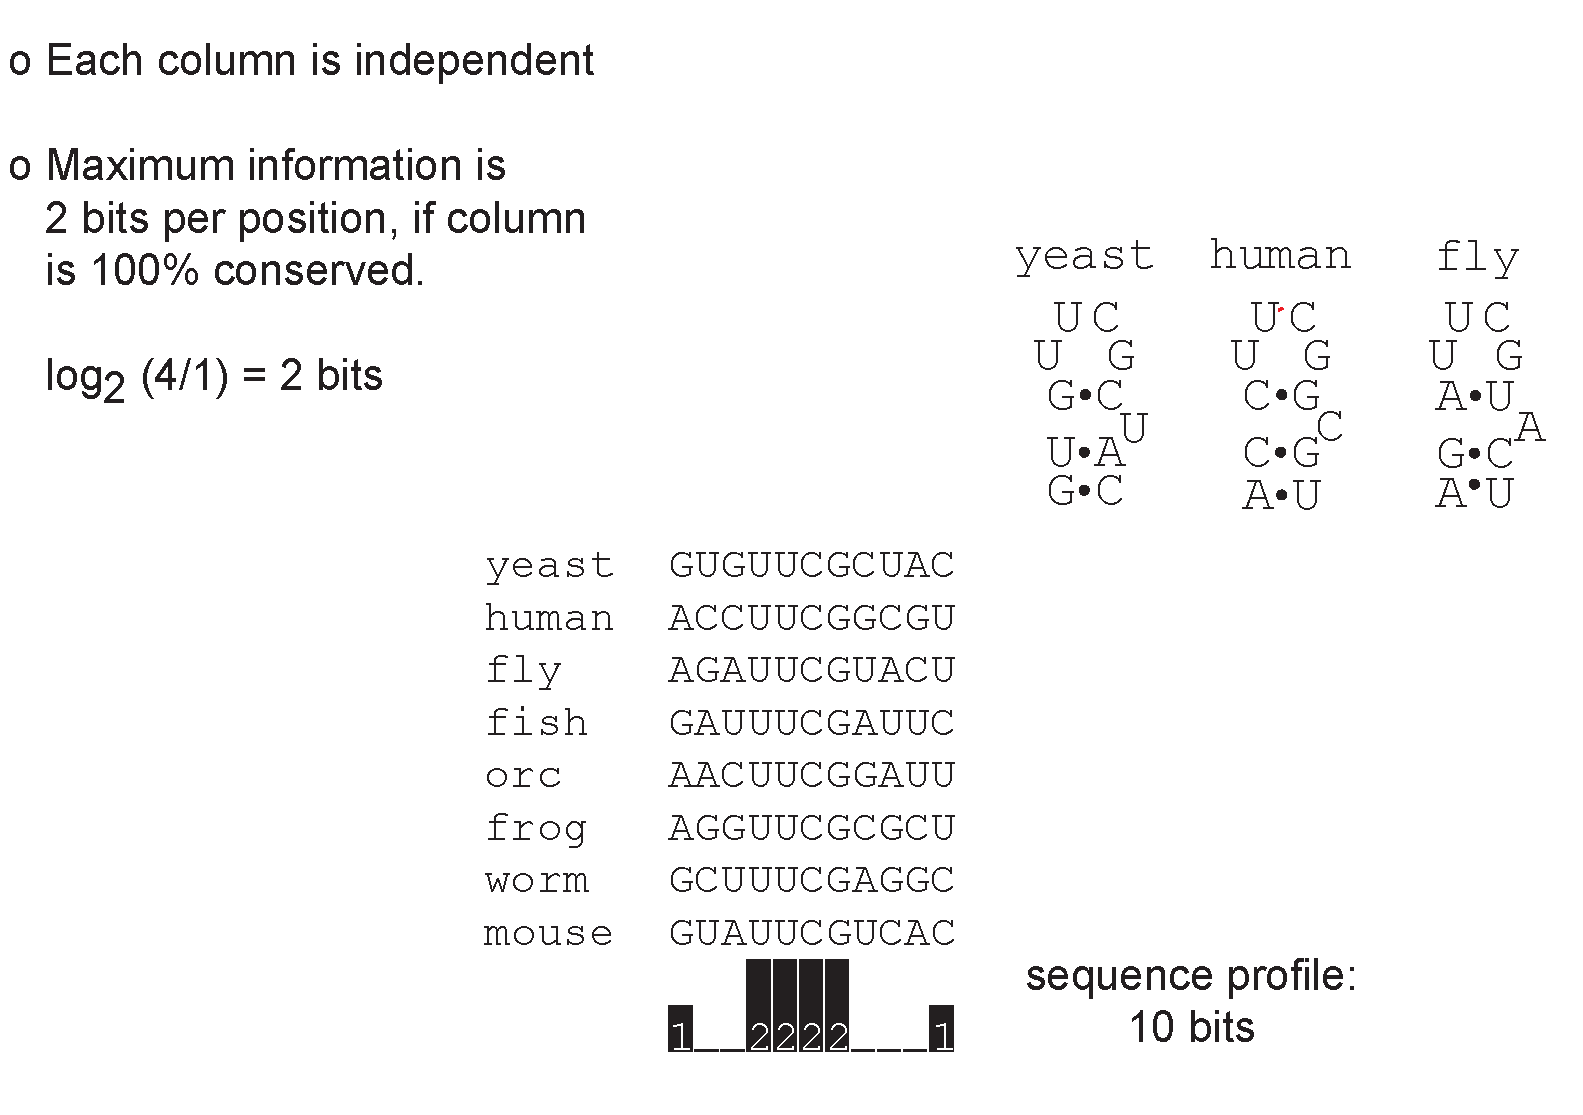
\includegraphics[width=10.5in]{figs/info_for_alignment_primary}
\end{center}

\end{slide}

%%%%%%%%%%%%%%%%%%%%%%%%%%%%%%%%%%%%%%%%%%%%%%%%%%%%%%%%%%%%%%%%%%%%%%
\begin{slide}
\begin{center}
\textbf{RNA alignment with sequence/structure profiles}
\end{center}
\medskip

\begin{center}
\includegraphics[width=10.5in]{figs/info_for_alignment_structure}
\end{center}

\end{slide}

%%%%%%%%%%%%%%%%%%%%%%%%%%%%%%%%%%%%%%%%%%%%%%%%%%%%%%%%%%%%%%%%%%%%%%
%%%%%%%%%%%%%%%%%%%%%%%%%%%%%%%%%%%%%%%%%%%%%%%%%%%%%%%%%%%%%%%%%%%%%%%%%%
%Slide 2 - SSU rRNA is very well conserved across all three domains
\begin{slide}
\begin{center}
\large
\textbf{Information in bacterial SSU}
\end{center}
%\vspace{0.5in}
\small
\hspace{1.0in}
\underline{primary sequence (about 2000 bits)}
\hspace{0.7in}
\underline{secondary structure (about 400 bits)}

\begin{center}
%\includegraphics[height=4.6in]{figs/ecoli_16S}
%\includegraphics[height=4.6in]{figs/mvan_16S}
%\includegraphics[height=4.6in]{figs/zmays_16S}
%\includegraphics[height=4.45in]{figs/bac_info}
%\includegraphics[height=4.45in]{figs/arc_info}
%\includegraphics[height=4.45in]{figs/euk_info}
\includegraphics[height=6in]{figs/bac_info}
\includegraphics[height=6in]{figs/bac_struct}
\end{center}

\begin{flushright}
\tiny{\texttt{Secondary structure diagrams created based}} \\
\tiny{\texttt{alignments and diagrams from:}} \\
\tiny{\texttt{URL:http://www.rna.icmb.utexas.edu/}}
\end{flushright}
%should this slide have a tree of life? if not where should it go?
\vfill
\end{slide}

%%%%%%%%%%%%%%%%%%%%%%%%%%%%%%%%%%%%%%%%%%%%%%%%%%%%%%%%%%%%%%%%%%%%%%%%%%
\begin{comment}
\begin{slide}
\begin{center}
\large
\textbf{Alignment using profiles}
\end{center}
\medskip
\small
\begin{itemize}
\item
\textbf{main idea:} use fast HMM when it's accurate, appealing to CM when it's not
\item
need some type of measure of confidence in regions of the HMM alignment
\item
requires some type of a \emph{map} from HMM to CM
\end{itemize}
\vfill
\end{slide}
\end{comment}
%%%%%%%%%%%%%%%%%%%%%%%%%%%%%%%%%%%%%%%%%%%%%%%%%%%%%%%%%%%%%%%%%%%%%%%%%%
\begin{slide}
\begin{center}
\large
\textbf{Accelerating CM alignment using HMMs}
\end{center}
\medskip
\begin{minipage}{6in}
\footnotesize
\begin{itemize}
\item
\textbf{main idea:} use fast HMM when it's accurate, appealing to CM when it's not
\item
%requires a method for determining the level of confidence
%(probability) that regions of the HMM alignment are correct 
%need to know the confidence level that regions of the HMM alignment
%are correct
need some type of measure of confidence in regions of the HMM alignment

\end{itemize}
\small
\hspace{0.3in}
\underline{HMM alignment}%\hspace{1.5in}---- $>$
\begin{itemize}
%\item
%each column of 2D dynamic programming \\ matrix corresponds to a column
%of the seed alignment
%\item
%each row of the matrix corresponds to a \\ position of the new sequence
\item
each column of the grid corresponds to a \\ column
of the seed alignment
\item
each row of the grid corresponds to a \\ position of the new sequence
\end{itemize}
\vspace{3in}
\end{minipage}
\begin{minipage}{4in}
\begin{center}
\includegraphics[height=6in]{figs/hmm_alignment2_layer1}
\end{center}
\vspace{1.5in}
\end{minipage}
\end{slide}
%%%%%%%%%%%%%%%%%%%%%%%%%%%%%%%%%%%%%
%%%%%%%%%%%%%%%%%%%%%%%%%%%%%%%%%%%%%%%%%%%%%%%%%%%%%%%%%%%%%%%%%%%%%%%%%%
\begin{slide}
\begin{center}
\large
\textbf{Accelerating CM alignment using HMMs}
\end{center}
\medskip
\begin{minipage}{6in}
\footnotesize
\begin{itemize}
\item
\textbf{main idea:} use fast HMM when it's accurate, appealing to CM when it's not
%for the regions of the alignment it can get right
%and use slower, more accurate CM for the rest
\item
%requires a method for determining the level of confidence
%(probability) that regions of the HMM alignment are correct 
%need to know the confidence level that regions of the HMM alignment
%are correct
need some type of measure of confidence in regions of the HMM alignment

\end{itemize}
\small
\hspace{0.3in}
\underline{HMM alignment}%\hspace{1.5in}---- $>$
\begin{itemize}
\item
each column of the grid corresponds to a \\ column
of the seed alignment
\item
each row of the grid corresponds to a \\ position of the new sequence
\end{itemize}
\vspace{3in}
\end{minipage}
\begin{minipage}{4in}
\begin{center}
\includegraphics[height=6in]{figs/hmm_alignment2_layer2}
\end{center}
\vspace{1.5in}
\end{minipage}
\end{slide}
%%%%%%%%%%%%%%%%%%%%%%%%%%%%%%%%%%%%%
%%%%%%%%%%%%%%%%%%%%%%%%%%%%%%%%%%%%%%%%%%%%%%%%%%%%%%%%%%%%%%%%%%%%%%%%%%
\begin{slide}
\begin{center}
\large
\textbf{Accelerating CM alignment using HMMs}
\end{center}
\medskip
\begin{minipage}{6in}
\footnotesize
\begin{itemize}
\item
\textbf{main idea:} use fast HMM when it's accurate, appealing to CM when it's not
%main idea: use fast HMM for the regions of the alignment it can get right
%and use slower, more accurate CM for the rest
\item
%requires a method for determining the level of confidence
%(probability) that regions of the HMM alignment are correct 
%need to know the confidence level that regions of the HMM alignment
%are correct
need some type of measure of confidence in regions of the HMM alignment

\end{itemize}
\small
\hspace{0.3in}
\underline{HMM alignment}%\hspace{1.5in}---- $>$
\begin{itemize}
\item
each column of the grid corresponds to a \\ column
of the seed alignment
\item
each row of the grid corresponds to a \\ position of the new sequence
\end{itemize}
\begin{center}
\normalsize
\textbf{How can we use this information during CM alignment?}
\end{center}
\vspace{1.9in}
\end{minipage}
\begin{minipage}{4in}
\begin{center}
\includegraphics[height=6in]{figs/hmm_alignment2_layer3}
\end{center}
\vspace{1.5in}
\end{minipage}
\end{slide}
%%%%%%%%%%%%%%%%%%%%%%%%%%%%%%%%%%%%%

%%%%%%%%%%%%%%%%%%%%%%%%%%%%%%%%%%%%%%%%%%%%%%%%%%%%%%%%%%%%%%%%%%%%%%%%%%
\begin{slide}
\begin{center}
\large
\textbf{Banded CMs}
%\textbf{How can we use this information during CM alignment?}
%\textbf{Accelerating CM alignment using HMMs}
\end{center}
\medskip
%\begin{minipage}{6in}
%\begin{center}
%\normalsize
%\textbf{How can we use this information during CM alignment?}
%\end{center}
\small
\begin{itemize}
\item
\textbf{main idea:} eliminate potential alignments the HMM tells us are very improbable
%\item
%restrict which cells of the CM dynamic programming matrix are filled in
%\item
%requires some type of \textbf{map} from the HMM to the CM
%\item
%each single stranded column or base pair from the seed alignment
%corresponds to \\ a face of the 3D CM dynamic programming matrix
\end{itemize}
\begin{center}
\includegraphics[width=8in]{figs/post_hmm_to_cm_map2_layer1}
\end{center}
\vfill
%\end{minipage}
%\begin{minipage}{4in}
%\vspace{.5in}
%\end{minipage}
\end{slide}
%%%%%%%%%%%%%%%%%%%%%%%%%%%%%%%%%%%%%
%%%%%%%%%%%%%%%%%%%%%%%%%%%%%%%%%%%%%%%%%%%%%%%%%%%%%%%%%%%%%%%%%%%%%%%%%%
\begin{slide}
\begin{center}
\large
\textbf{Banded CMs}
%\textbf{How can we use this information during CM alignment?}
%\textbf{Accelerating CM alignment using HMMs}
\end{center}
\medskip
%\begin{minipage}{6in}
%\begin{center}
%\normalsize
%\textbf{How can we use this information during CM alignment?}
%\end{center}
\small
\begin{itemize}
\item
\textbf{main idea:} eliminate potential alignments the HMM tells us are very improbable
%\item
%restrict which cells of the CM dynamic programming matrix are filled in
%\item
%requires some type of \textbf{map} from the HMM to the CM
%\item
%each single stranded column or base pair from the seed alignment
%corresponds to \\ a face of the 3D CM dynamic programming matrix
\end{itemize}
\begin{center}
\includegraphics[width=8in]{figs/post_hmm_to_cm_map2_layer2}
\end{center}
\vfill
%\end{minipage}
%\begin{minipage}{4in}
%\vspace{.5in}
%\end{minipage}
\end{slide}
%%%%%%%%%%%%%%%%%%%%%%%%%%%%%%%%%%%%%
%%%%%%%%%%%%%%%%%%%%%%%%%%%%%%%%%%%%%%%%%%%%%%%%%%%%%%%%%%%%%%%%%%%%%%%%%%
\begin{slide}
\begin{center}
\large
\textbf{Banded CMs}
%\textbf{How can we use this information during CM alignment?}
%\textbf{Accelerating CM alignment using HMMs}
\end{center}
\medskip
%\begin{minipage}{6in}
%\begin{center}
%\normalsize
%\textbf{How can we use this information during CM alignment?}
%\end{center}
\small
\begin{itemize}
\item
\textbf{main idea:} eliminate potential alignments the HMM tells us are very improbable
%\item
%restrict which cells of the CM dynamic programming matrix are filled in
%\item
%requires some type of \textbf{map} from the HMM to the CM
%\item
%each single stranded column or base pair from the seed alignment
%corresponds to \\ a face of the 3D CM dynamic programming matrix
\end{itemize}
\begin{center}
\includegraphics[width=8in]{figs/post_hmm_to_cm_map2_layer3}
\end{center}
\vfill
%\end{minipage}
%\begin{minipage}{4in}
%\vspace{.5in}
%\end{minipage}
\end{slide}
%%%%%%%%%%%%%%%%%%%%%%%%%%%%%%%%%%%%%%%%%%%%%%%%%%%%%%%%%%%%%%%%%%%%%%%%%%
%%%%%%%%%%%%%%%%%%%%%%%%%%%%%%%%%%%%%%%%%%%%%%%%%%%%%%%%%%%%%%%%%%%%%%%%%%
\begin{slide}
\begin{center}
\large
\textbf{Banded CMs}
%\textbf{How can we use this information during CM alignment?}
%\textbf{Accelerating CM alignment using HMMs}
\end{center}
\medskip
%\begin{minipage}{6in}
%\begin{center}
%\normalsize
%\textbf{How can we use this information during CM alignment?}
%\end{center}
\small
\begin{itemize}
\item
\textbf{main idea:} eliminate potential alignments the HMM tells us are very improbable
%\item
%restrict which cells of the CM dynamic programming matrix are filled in
%\item
%requires some type of \textbf{map} from the HMM to the CM
%\item
%each single stranded column or base pair from the seed alignment
%corresponds to \\ a face of the 3D CM dynamic programming matrix
\end{itemize}
\begin{center}
\includegraphics[width=8in]{figs/post_hmm_to_cm_map2_layer4}
\end{center}
\vfill
%\end{minipage}
%\begin{minipage}{4in}
%\vspace{.5in}
%\end{minipage}
\end{slide}
%%%%%%%%%%%%%%%%%%%%%%%%%%%%%%%%%%%%%%%%%%%%%%%%%%%%%%%%%%%%%%%%%%%%%%%%%%
%%%%%%%%%%%%%%%%%%%%%%%%%%%%%%%%%%%%%%%%%%%%%%%%%%%%%%%%%%%%%%%%%%%%%%%%%%
\begin{slide}
\begin{center}
\large
\textbf{Banded CMs}
%\textbf{How can we use this information during CM alignment?}
%\textbf{Accelerating CM alignment using HMMs}
\end{center}
\medskip
%\begin{minipage}{6in}
%\begin{center}
%\normalsize
%\textbf{How can we use this information during CM alignment?}
%\end{center}
\small
\begin{itemize}
\item
\textbf{main idea:} eliminate potential alignments the HMM tells us are very improbable
%\item
%restrict which cells of the CM dynamic programming matrix are filled in
%\item
%requires some type of \textbf{map} from the HMM to the CM
%\item
%each single stranded column or base pair from the seed alignment
%corresponds to \\ a face of the 3D CM dynamic programming matrix
\end{itemize}
\begin{center}
\includegraphics[width=8in]{figs/post_hmm_to_cm_map2_layer5}
\end{center}
\vfill
%\end{minipage}
%\begin{minipage}{4in}
%\vspace{.5in}
%\end{minipage}
\end{slide}
%%%%%%%%%%%%%%%%%%%%%%%%%%%%%%%%%%%%%%%%%%%%%%%%%%%%%%%%%%%%%%%%%%%%%%%%%%
%%%%%%%%%%%%%%%%%%%%%%%%%%%%%%%%%%%%%%%%%%%%%%%%%%%%%%%%%%%%%%%%%%%%%%%%%%
\begin{slide}
\begin{center}
\large
\textbf{Banded CMs}
%\textbf{How can we use this information during CM alignment?}
%\textbf{Accelerating CM alignment using HMMs}
\end{center}
\medskip
%\begin{minipage}{6in}
%\begin{center}
%\normalsize
%\textbf{How can we use this information during CM alignment?}
%\end{center}
\small
\begin{itemize}
\item
\textbf{main idea:} eliminate potential alignments the HMM tells us are very improbable
%\item
%restrict which cells of the CM dynamic programming matrix are filled in
%\item
%requires some type of \textbf{map} from the HMM to the CM
%\item
%each single stranded column or base pair from the seed alignment
%corresponds to \\ a face of the 3D CM dynamic programming matrix
\end{itemize}
\begin{center}
\includegraphics[width=8in]{figs/post_hmm_to_cm_map2_layer6}
\end{center}
\vfill
%\end{minipage}
%\begin{minipage}{4in}
%\vspace{.5in}
%\end{minipage}
\end{slide}
%%%%%%%%%%%%%%%%%%%%%%%%%%%%%%%%%%%%%%%%%%%%%%%%%%%%%%%%%%%%%%%%%%%%%%%%%%
%%%%%%%%%%%%%%%%%%%%%%%%%%%%%%%%%%%%%%%%%%%%%%%%%%%%%%%%%%%%%%%%%%%%%%%%%%
\begin{slide}
\begin{center}
\large
\textbf{Banded CMs}
%\textbf{How can we use this information during CM alignment?}
%\textbf{Accelerating CM alignment using HMMs}
\end{center}
\medskip
%\begin{minipage}{6in}
%\begin{center}
%\normalsize
%\textbf{How can we use this information during CM alignment?}
%\end{center}
\small
\begin{itemize}
\item
\textbf{main idea:} eliminate potential alignments the HMM tells us are very improbable
%\item
%restrict which cells of the CM dynamic programming matrix are filled in
%\item
%requires some type of \textbf{map} from the HMM to the CM
%\item
%each single stranded column or base pair from the seed alignment
%corresponds to \\ a face of the 3D CM dynamic programming matrix
\end{itemize}
\begin{center}
\includegraphics[width=8in]{figs/post_hmm_to_cm_map2_layer7}
\end{center}
\vfill
%\end{minipage}
%\begin{minipage}{4in}
%\vspace{.5in}
%\end{minipage}
\end{slide}
%%%%%%%%%%%%%%%%%%%%%%%%%%%%%%%%%%%%%%%%%%%%%%%%%%%%%%%%%%%%%%%%%%%%%%%%%%
%%%%%%%%%%%%%%%%%%%%%%%%%%%%%%%%%%%%%%%%%%%%%%%%%%%%%%%%%%%%%%%%%%%%%%%%%%
\begin{slide}
\begin{center}
\large
\textbf{Banded CMs}
%\textbf{How can we use this information during CM alignment?}
%\textbf{Accelerating CM alignment using HMMs}
\end{center}
\medskip
%\begin{minipage}{6in}
%\begin{center}
%\normalsize
%\textbf{How can we use this information during CM alignment?}
%\end{center}
\small
\begin{itemize}
\item
\textbf{main idea:} eliminate potential alignments the HMM tells us are very improbable
%\item
%restrict which cells of the CM dynamic programming matrix are filled in
%\item
%requires some type of \textbf{map} from the HMM to the CM
%\item
%each single stranded column or base pair from the seed alignment
%corresponds to \\ a face of the 3D CM dynamic programming matrix
\end{itemize}
\begin{center}
\includegraphics[width=8in]{figs/post_hmm_to_cm_map2_layer8}
\end{center}
\vfill
%\end{minipage}
%\begin{minipage}{4in}
%\vspace{.5in}
%\end{minipage}
\end{slide}
%%%%%%%%%%%%%%%%%%%%%%%%%%%%%%%%%%%%%%%%%%%%%%%%%%%%%%%%%%%%%%%%%%%%%%%%%%
%%%%%%%%%%%%%%%%%%%%%%%%%%%%%%%%%%%%%%%%%%%%%%%%%%%%%%%%%%%%%%%%%%%%%%%%%%
\begin{slide}
\begin{center}
\large
\textbf{Banded CMs}
%\textbf{How can we use this information during CM alignment?}
%\textbf{Accelerating CM alignment using HMMs}
\end{center}
\medskip
%\begin{minipage}{6in}
%\begin{center}
%\normalsize
%\textbf{How can we use this information during CM alignment?}
%\end{center}
\small
\begin{itemize}
\item
\textbf{main idea:} eliminate potential alignments the HMM tells us are very improbable
%\item
%restrict which cells of the CM dynamic programming matrix are filled in
%\item
%requires some type of \textbf{map} from the HMM to the CM
%\item
%each single stranded column or base pair from the seed alignment
%corresponds to \\ a face of the 3D CM dynamic programming matrix
\end{itemize}
\begin{center}
\includegraphics[width=8in]{figs/post_hmm_to_cm_map2_layer9}
\end{center}
\vfill
%\end{minipage}
%\begin{minipage}{4in}
%\vspace{.5in}
%\end{minipage}
\end{slide}
%%%%%%%%%%%%%%%%%%%%%%%%%%%%%%%%%%%%%%%%%%%%%%%%%%%%%%%%%%%%%%%%%%%%%%%%%%
%%%%%%%%%%%%%%%%%%%%%%%%%%%%%%%%%%%%%%%%%%%%%%%%%%%%%%%%%%%%%%%%%%%%%%%%%%
\begin{slide}
\begin{center}
\large
\textbf{Banded CMs}
%\textbf{How can we use this information during CM alignment?}
%\textbf{Accelerating CM alignment using HMMs}
\end{center}
\medskip
%\begin{minipage}{6in}
%\begin{center}
%\normalsize
%\textbf{How can we use this information during CM alignment?}
%\end{center}
\small
\begin{itemize}
\item
\textbf{main idea:} eliminate potential alignments the HMM tells us are very improbable
%\item
%restrict which cells of the CM dynamic programming matrix are filled in
%\item
%requires some type of \textbf{map} from the HMM to the CM
%\item
%each single stranded column or base pair from the seed alignment
%corresponds to \\ a face of the 3D CM dynamic programming matrix
\end{itemize}
\begin{center}
\includegraphics[width=8in]{figs/post_hmm_to_cm_map2_layer10}
\end{center}
\vfill
%\end{minipage}
%\begin{minipage}{4in}
%\vspace{.5in}
%\end{minipage}
\end{slide}
%%%%%%%%%%%%%%%%%%%%%%%%%%%%%%%%%%%%%%%%%%%%%%%%%%%%%%%%%%%%%%%%%%%%%%%%%%
%%%%%%%%%%%%%%%%%%%%%%%%%%%%%%%%%%%%%%%%%%%%%%%%%%%%%%%%%%%%%%%%%%%%%%%%%%
\begin{slide}
\begin{center}
\large
\textbf{Banded CMs}
%\textbf{How can we use this information during CM alignment?}
%\textbf{Accelerating CM alignment using HMMs}
\end{center}
\medskip
%\begin{minipage}{6in}
%\begin{center}
%\normalsize
%\textbf{How can we use this information during CM alignment?}
%\end{center}
\small
\begin{itemize}
\item
\textbf{main idea:} eliminate potential alignments the HMM tells us are very improbable
%\item
%restrict which cells of the CM dynamic programming matrix are filled in
%\item
%requires some type of \textbf{map} from the HMM to the CM
%\item
%each single stranded column or base pair from the seed alignment
%corresponds to \\ a face of the 3D CM dynamic programming matrix
\end{itemize}
\begin{center}
\includegraphics[width=8in]{figs/post_hmm_to_cm_map2_layer11}
\end{center}
\vfill
%\end{minipage}
%\begin{minipage}{4in}
%\vspace{.5in}
%\end{minipage}
\end{slide}
%%%%%%%%%%%%%%%%%%%%%%%%%%%%%%%%%%%%%%%%%%%%%%%%%%%%%%%%%%%%%%%%%%%%%%%%%%
%%%%%%%%%%%%%%%%%%%%%%%%%%%%%%%%%%%%%%%%%%%%%%%%%%%%%%%%%%%%%%%%%%%%%%%%%%
\begin{slide}
\begin{center}
\large
\textbf{Banded CMs}
%\textbf{How can we use this information during CM alignment?}
%\textbf{Accelerating CM alignment using HMMs}
\end{center}
\medskip
%\begin{minipage}{6in}
%\begin{center}
%\normalsize
%\textbf{How can we use this information during CM alignment?}
%\end{center}
\small
\begin{itemize}
\item
\textbf{main idea:} eliminate potential alignments the HMM tells us are very improbable
%\item
%restrict which cells of the CM dynamic programming matrix are filled in
%\item
%requires some type of \textbf{map} from the HMM to the CM
%\item
%each single stranded column or base pair from the seed alignment
%corresponds to \\ a face of the 3D CM dynamic programming matrix
\end{itemize}
\begin{center}
\includegraphics[width=8in]{figs/post_hmm_to_cm_map2_layer12}
\end{center}
\vfill
%\end{minipage}
%\begin{minipage}{4in}
%\vspace{.5in}
%\end{minipage}
\end{slide}
%%%%%%%%%%%%%%%%%%%%%%%%%%%%%%%%%%%%%%%%%%%%%%%%%%%%%%%%%%%%%%%%%%%%%%%%%%
%%%%%%%%%%%%%%%%%%%%%%%%%%%%%%%%%%%%%%%%%%%%%%%%%%%%%%%%%%%%%%%%%%%%%%%%%%
\begin{slide}
\begin{center}
\large
\textbf{Banded CMs}
%\textbf{How can we use this information during CM alignment?}
%\textbf{Accelerating CM alignment using HMMs}
\end{center}
\medskip
%\begin{minipage}{6in}
%\begin{center}
%\normalsize
%\textbf{How can we use this information during CM alignment?}
%\end{center}
\small
\begin{itemize}
\item
\textbf{main idea:} eliminate potential alignments the HMM tells us are very improbable
%\item
%restrict which cells of the CM dynamic programming matrix are filled in
%\item
%requires some type of \textbf{map} from the HMM to the CM
%\item
%each single stranded column or base pair from the seed alignment
%corresponds to \\ a face of the 3D CM dynamic programming matrix
\end{itemize}
\begin{center}
\includegraphics[width=8in]{figs/post_hmm_to_cm_map2_layer13}
\end{center}
\vfill
%\end{minipage}
%\begin{minipage}{4in}
%\vspace{.5in}
%\end{minipage}
\end{slide}
%%%%%%%%%%%%%%%%%%%%%%%%%%%%%%%%%%%%%%%%%%%%%%%%%%%%%%%%%%%%%%%%%%%%%%%%%%
%%%%%%%%%%%%%%%%%%%%%%%%%%%%%%%%%%%%%%%%%%%%%%%%%%%%%%%%%%%%%%%%%%%%%%%%%%
\begin{slide}
\begin{center}
\large
\textbf{Banded CMs}
%\textbf{How can we use this information during CM alignment?}
%\textbf{Accelerating CM alignment using HMMs}
\end{center}
\medskip
%\begin{minipage}{6in}
%\begin{center}
%\normalsize
%\textbf{How can we use this information during CM alignment?}
%\end{center}
\small
\begin{itemize}
\item
\textbf{main idea:} eliminate potential alignments the HMM tells us are very improbable
%\item
%restrict which cells of the CM dynamic programming matrix are filled in
%\item
%requires some type of \textbf{map} from the HMM to the CM
%\item
%each single stranded column or base pair from the seed alignment
%corresponds to \\ a face of the 3D CM dynamic programming matrix
\end{itemize}
\begin{center}
\includegraphics[width=8in]{figs/post_hmm_to_cm_map2_layer14}
\end{center}
\vfill
%\end{minipage}
%\begin{minipage}{4in}
%\vspace{.5in}
%\end{minipage}
\end{slide}
%%%%%%%%%%%%%%%%%%%%%%%%%%%%%%%%%%%%%%%%%%%%%%%%%%%%%%%%%%%%%%%%%%%%%%%%%%
%%%%%%%%%%%%%%%%%%%%%%%%%%%%%%%%%%%%%%%%%%%%%%%%%%%%%%%%%%%%%%%%%%%%%%%%%%
\begin{slide}
\begin{center}
\large
\textbf{Banded CMs}
%\textbf{How can we use this information during CM alignment?}
%\textbf{Accelerating CM alignment using HMMs}
\end{center}
\medskip
%\begin{minipage}{6in}
%\begin{center}
%\normalsize
%\textbf{How can we use this information during CM alignment?}
%\end{center}
\small
\begin{itemize}
\item
\textbf{main idea:} eliminate potential alignments the HMM tells us are very improbable
%\item
%restrict which cells of the CM dynamic programming matrix are filled in
%\item
%requires some type of \textbf{map} from the HMM to the CM
%\item
%each single stranded column or base pair from the seed alignment
%corresponds to \\ a face of the 3D CM dynamic programming matrix
\end{itemize}
\begin{center}
\includegraphics[width=8in]{figs/post_hmm_to_cm_map2_layer15}
\end{center}
\vfill
%\end{minipage}
%\begin{minipage}{4in}
%\vspace{.5in}
%\end{minipage}
\end{slide}
%%%%%%%%%%%%%%%%%%%%%%%%%%%%%%%%%%%%%%%%%%%%%%%%%%%%%%%%%%%%%%%%%%%%%%%%%%
%%%%%%%%%%%%%%%%%%%%%%%%%%%%%%%%%%%%%%%%%%%%%%%%%%%%%%%%%%%%%%%%%%%%%%%%%%
\begin{slide}
\begin{center}
\large
\textbf{Banded CMs}
%\textbf{How can we use this information during CM alignment?}
%\textbf{Accelerating CM alignment using HMMs}
\end{center}
\medskip
%\begin{minipage}{6in}
%\begin{center}
%\normalsize
%\textbf{How can we use this information during CM alignment?}
%\end{center}
\small
\begin{itemize}
\item
\textbf{main idea:} eliminate potential alignments the HMM tells us are very improbable
%\item
%restrict which cells of the CM dynamic programming matrix are filled in
%\item
%requires some type of \textbf{map} from the HMM to the CM
%\item
%each single stranded column or base pair from the seed alignment
%corresponds to \\ a face of the 3D CM dynamic programming matrix
\end{itemize}
\begin{center}
\includegraphics[width=8in]{figs/post_hmm_to_cm_map2_layer16}
\end{center}
\vfill
%\end{minipage}
%\begin{minipage}{4in}
%\vspace{.5in}
%\end{minipage}
\end{slide}
%%%%%%%%%%%%%%%%%%%%%%%%%%%%%%%%%%%%%%%%%%%%%%%%%%%%%%%%%%%%%%%%%%%%%%%%%%
%%%%%%%%%%%%%%%%%%%%%%%%%%%%%%%%%%%%%
%Stats in this slide from files in
%/nfs/wol2/people/nawrocki/notebook/6_0201_friday_talk/cells_saved_dir
%and logged in ~/notebook/6_0201_friday_talk/00LOG
\begin{comment}
\begin{slide}
\begin{center}
%\large
\textbf{HMM banded approach offers significant acceleration}
\end{center}
\medskip

\begin{center}
\begin{small}
\begin{tabular}{crrrr} %\hline
& \multicolumn{1}{c}{average} & & & potential \\ 
family & length (nt) & total cells & banded cells & speed-up\textbf{*} \\ \hline
\multicolumn{5}{c}{} \\
tRNA & 73 & 656,951 & 9,071.3 & 72.4 \\ %0.75 gap thresh b6
%tRNA & 73 & 1.0 X 10$^6$ & 6,603 & 157.1 \\ %1.0 gap thresh b4
\multicolumn{5}{c}{} \\
RNase P & 332 & 5.8 X 10$^7$ & 143,738.6 & 406.2 \\  %0.75 gap thresh b6
%RNase P & 332 & 2.4 X 10$^8$ & 359,815 & 665.6 \\ %1.0 gap thresh
\multicolumn{5}{c}{} \\
%SSU rRNA & 1531 & 6.3 X 10$^9$ & 266,128 & 23,828.05 \\ %1.0 gap thresh
SSU rRNA & 1531 & 5.7 X 10$^9$ & 199,604.2 & 28,487.2 \\ %0.75 gap thresh b4
(bacteria) & & & & \\
\multicolumn{5}{c}{} \\
\end{tabular}
\end{small}
\end{center}
\tiny
\begin{center}
\texttt{\textbf{* does not consider time required for HMM alignment}}
\end{center}
\vfill
\end{slide}
\end{comment}
%\begin{tabular}{|c|r|r|r|r|} \hline
%family & avg length (nt) & total cells & banded cells & potential speed-up \\ \hline
%\hline
%tRNA & 73 & 16,571 & 4,752 & 3.5  \\ \hline
%RNase P & 377 & 440,336 & 53,990 & 8.2  \\ \hline
%16S rRNA & 1540 & 7,258,785 & 200,937 & 36.1 \\ \hline
%%%%%%%%%%%%%%%%%%%%%%%%%%%%%%%%%%%%%%%%%%%%%%%%%%%%%%%%%%%%%%%%%%%%%%%%%%
%%%%%%%%%%%%%%%%%%%%%%%%%%%%%%%%%%%%%

%%%%%%%%%%%%%%%%%%%%%%%%%%%%%%%%%%%%%%%%%%%%%%%%%%%%%%%%%%%%%%%%%%%
\begin{slide}
\begin{center}
\large
\textbf{Benchmarking SSU alignment}
\end{center}
\medskip

\small
\begin{itemize}
\item
Does the banded CM approach sacrifice accuracy relative to
non-banded CM alignment?
%\item
%How accurately do profiles align SSU?
%\end{itemize}
\item
'Gold standard' testing dataset
\begin{itemize}
\item
structural alignment of 152 bacterial SSU sequences
from Robin Gutell's database
%the Comparative RNA Website (CRW)
%structural alignment of 221 bacterial SSU sequences
%from the Comparative RNA Website (CRW)
\item
this is the CRW bacterial seed alignment filtered to 92\% identity
\item
determined by 'manual' comparative analysis
\begin{comment}
\item
152 deep alignment is clustered into two groups based on sequence identity:
%representative subset of 46 sequences used as the seed alignment
%(no two are $>$ 80\% identical)
\begin{itemize}
\item
training (seed) alignment of 101 sequences
\item
testing alignment of 51 sequences
\item
  no train/test pair is > 80\% identical
\end{itemize}
\item
Benchmark: train profile on 101-deep seed and test alignment accuracy on the remaining 175 sequences
\end{comment}

%measure accuracy of predicted base pairs versus correct base pairs
\end{itemize}
\end{itemize}

\center{\includegraphics[width=10.5in]{figs/diana_benchmark_l1}}

\vfill
\end{slide}
%%%%%%%%%%%%%%%%%%%%%%%%%%%%%%%%%%%%%%%%%%%%%%%%%%%%%%%%%%%%%%%%%%%%%%%%%
%%%%%%%%%%%%%%%%%%%%%%%%%%%%%%%%%%%%%%%%%%%%%%%%%%%%%%%%%%%%%%%%%%%
\begin{slide}
\begin{center}
\large
\textbf{Benchmarking SSU alignment}
\end{center}
\medskip

\small
\begin{itemize}
\item
Does the banded CM approach sacrifice accuracy relative to
non-banded CM alignment?
%\item
%How accurately do profiles align SSU?
%\end{itemize}
\item
'Gold standard' testing dataset
\begin{itemize}
\item
structural alignment of 152 bacterial SSU sequences
from Robin Gutell's database
%the Comparative RNA Website (CRW)
%structural alignment of 221 bacterial SSU sequences
%from the Comparative RNA Website (CRW)
\item
this is the CRW bacterial seed alignment filtered to 92\% identity
\item
determined by 'manual' comparative analysis
\begin{comment}
\item
152 deep alignment is clustered into two groups based on sequence identity:
%representative subset of 46 sequences used as the seed alignment
%(no two are $>$ 80\% identical)
\begin{itemize}
\item
training (seed) alignment of 101 sequences
\item
testing alignment of 51 sequences
\item
  no train/test pair is > 80\% identical
\end{itemize}
\item
Benchmark: train profile on 101-deep seed and test alignment accuracy on the remaining 175 sequences
\end{comment}

%measure accuracy of predicted base pairs versus correct base pairs
\end{itemize}
\end{itemize}

\center{\includegraphics[width=10.5in]{figs/diana_benchmark_l2}}

\vfill
\end{slide}
%%%%%%%%%%%%%%%%%%%%%%%%%%%%%%%%%%%%%%%%%%%%%%%%%%%%%%%%%%%%%%%%%%%%%%%%%

%%%%%%%%%%%%%%%%%%%%%%%%%%%%%%%%%%%%%%%%%%%%%%%%%%%%%%%%%%%%%%%%%%%%%%%%%
% Results pre 09.19.07 (reported in Venter, AG, Friday talk)
%HMMs & 96.62\% & 0.1 (pre 09.19.07) 
%non-banded CMs & 98.19\% & 1407.1 (pre 09.19.07)\\ 
%HMM banded CMs & 98.17\% & 3.5 \\ 
%
%%%%%%%%%%%%%%%%%%%%%%%%%%%%%%%%%%%%%%%%%%%%%%%%%%%%%%%%%%%%%%%%%%%%%%%%%
\begin{slide}
\begin{center}
\large
\textbf{Results}
\end{center}
\medskip
\medskip
\begin{center}

\begin{tabular}{rcr} 
& \multicolumn{1}{c}{alignment} & \multicolumn{1}{c}{time} \\
& \multicolumn{1}{c}{accuracy} & \multicolumn{1}{c}{(sec/seq)} \\ \hline
& \multicolumn{1}{c}{} & \multicolumn{1}{c}{} \\
clustalw & 92.2\% & 30.0 \\ 
& \multicolumn{1}{c}{} & \multicolumn{1}{c}{} \\
HMMs & 96.2\% & 0.08 \\ 
& \multicolumn{1}{c}{} & \multicolumn{1}{c}{} \\
non-banded CMs & 97.8\% & 780.0 \\ 
& \multicolumn{1}{c}{} & \multicolumn{1}{c}{} \\
%HMM banded CMs & 98.0\% & 1.3 \\ %1.1
%& \multicolumn{1}{c}{} & \multicolumn{1}{c}{} \\
\end{tabular}
\end{center}

\vfill
\end{slide}
%%%%%%%%%%%%%%%%%%%%%%%%%%%%%%%%%%%%%%%%%%%%%%%%%%%%%%%%%%%%%%%%%%%%%%%%%
%%%%%%%%%%%%%%%%%%%%%%%%%%%%%%%%%%%%%%%%%%%%%%%%%%%%%%%%%%%%%%%%%%%%%%%%%
\begin{slide}
\begin{center}
\large
\textbf{Results}
\end{center}
\medskip
\medskip
\begin{center}

\begin{tabular}{rcr} 
& \multicolumn{1}{c}{alignment} & \multicolumn{1}{c}{time} \\
& \multicolumn{1}{c}{accuracy} & \multicolumn{1}{c}{(sec/seq)} \\ \hline
& \multicolumn{1}{c}{} & \multicolumn{1}{c}{} \\
clustalw & 92.2\% & 30.0 \\ 
& \multicolumn{1}{c}{} & \multicolumn{1}{c}{} \\
HMMs & 96.2\% & 0.08 \\ 
& \multicolumn{1}{c}{} & \multicolumn{1}{c}{} \\
non-banded CMs & 97.8\% & 780.0 \\ 
& \multicolumn{1}{c}{} & \multicolumn{1}{c}{} \\
HMM banded CMs & 98.0\% & 1.3 \\ %1.1
& \multicolumn{1}{c}{} & \multicolumn{1}{c}{} \\
\end{tabular}
\end{center}

\vfill
\end{slide}
%%%%%%%%%%%%%%%%%%%%%%%%%%%%%%%%%%%%%%%%%%%%%%%%%%%%%%%%%%%%%%%%%%%%%%%%%
\begin{slide}
\begin{center}
\large
\textbf{Results}
\end{center}
\medskip
\medskip
\begin{center}

\begin{tabular}{rcr} 
& \multicolumn{1}{c}{alignment} & \multicolumn{1}{c}{time} \\
& \multicolumn{1}{c}{accuracy} & \multicolumn{1}{c}{(sec/seq)} \\ \hline
& \multicolumn{1}{c}{} & \multicolumn{1}{c}{} \\
clustalw & 92.2\% & 30.0 \\ 
& \multicolumn{1}{c}{} & \multicolumn{1}{c}{} \\
HMMs & 96.2\% & 0.08 \\ 
& \multicolumn{1}{c}{} & \multicolumn{1}{c}{} \\
non-banded CMs & 97.8\% & 780.0 \\ 
& \multicolumn{1}{c}{} & \multicolumn{1}{c}{} \\
HMM banded CMs & 98.0\% & 1.3 \\ %1.1
& \multicolumn{1}{c}{} & \multicolumn{1}{c}{} \\
\end{tabular}
\end{center}

\begin{center}
\large
\textbf{HMM banding technique is general}
\end{center}

%\small
%\begin{itemize}
%\item
%  Acceleration is greater for longer families
%\item
%  LSU alignment goes from about 3 hours to 8 seconds
%\end{itemize}

\small
\begin{center}
\begin{tabular}{lrr} 
%        clen    acceleration
%tRNA    72      4.5
%RNaseP  307     31.6
%SSU     1534    793.1  (no --sub) 396.5 (--sub)
%LSU     2916    3465.2 (no --sub)       
%see ~/notebook/7_0919_colorado_talk/00LOG:
  family & length & HMM banding acceleration \\ \hline
  \\
  tRNA   & 73     & 4.5 \\
  RNaseP bac A & 307 & 31.6 \\
  SSU & 1534 & 600.0 \\ %793.1
  LSU & 2914 & 1732.6 \\ %3465.2
\end{tabular}
\end{center}

\vfill
\end{slide}

%%%%%%%%%%%%%%%%%%%%%%%%%%%%%%%%%%%%%%%%%%%%%%%%%%%%%%%%%%%%%%%%%%%%%%%%%%
\begin{slide}
\begin{center}
\large
\textbf{NAST aligner}
\end{center}

\center{\includegraphics[width=10.5in]{figs/NN_v_Profile_NASTintro}}

\vfill
\end{slide}
%%%%%%%%%%%%%%%%%%%%%%%%%%%%%%%%%%%%%%%%%%%%%%%%%%%%%%%%%%%%%%%%%%%%%%%%%%
\begin{slide}
\begin{center}
\large
\textbf{Results: using NAST core alignment as seed}
\end{center}
\medskip
\medskip
\begin{center}

\begin{tabular}{rcc} 
& \multicolumn{1}{c}{alignment} & \multicolumn{1}{c}{time} \\
& \multicolumn{1}{c}{accuracy} & \multicolumn{1}{c}{(sec/seq)} \\ \hline
& \multicolumn{1}{c}{} & \multicolumn{1}{c}{} \\
NAST & 95.5\% & 6 \\ 
& \multicolumn{1}{c}{} & \multicolumn{1}{c}{} \\
HMMs & 96.2\% & 0.08 \\ 
%& \multicolumn{1}{c}{} & \multicolumn{1}{c}{} \\
%non-banded CMs & 97.3\% & 822.2 \\ 
& \multicolumn{1}{c}{} & \multicolumn{1}{c}{} \\
HMM banded CMs & 97.3\% & 1.3 \\ 
& \multicolumn{1}{c}{} & \multicolumn{1}{c}{} \\
\end{tabular}
\end{center}
\vfill
\end{slide}
%%%%%%%%%%%%%%%%%%%%%%%%%%%%%%%%%%%%%%%%%%%%%%%%%%%%%%%%%%%%%%%%%%%

%%%%%%%%%%%%%%%%%%%%%%%%%%%%%%%%%%%%%%%%%%%%%%%%%%%%%%%%%%%%%%%%%%%%%%%%%%
\begin{slide}
\begin{center}
\large
\textbf{NAST and Profiles}
\end{center}

\center{\includegraphics[width=10.5in]{figs/NAST_v_Profile}}

\vfill
\end{slide}
%%%%%%%%%%%%%%%%%%%%%%%%%%%%%%%%%%%%%%%%%%%%%%%%%%%%%%%%%%%%%%%%%%%%%%%%%%
\begin{slide}
\begin{center}
\large
\textbf{NAST and Profiles}
\end{center}

\center{\includegraphics[width=10.5in]{figs/NAST_v_SSUalign}}

\vfill
\end{slide}
%%%%%%%%%%%%%%%%%%%%%%%%%%%%%%%%%%%%%%%%%%%%%%%%%%%%%%%%%%%%%%%%%%%%%%%%%%


%%%%%%%%%%%%%%%%%%%%%%%%%%%%%%%%%%%%%%%%%%%%%%%%%%%%%%%%%%%%%%%%%%%%%%%%%
\begin{slide}
\begin{center}
\large
\textbf{Other features}
\end{center}

\small
\begin{itemize}
\item
partial sequence handling
\item
confidence estimates for each aligned residue
\item
easy parallelization with MPI
\item
future goals:
\begin{itemize}
\item
better test sets/benchmarks: how does alignment accuracy affect
phylogenetic \\ inference?
\item
meta-profile strategy
\item
more trustworthy seed alignments
%\item
%filters for misalignments and possibly chimeras
\end{itemize}
\end{itemize}

\center{\includegraphics[height=1.5in]{figs/infernal_logo}}


\begin{center}
\large{\textbf{Acknowledgements}}
\end{center}

%\footnotesize
%\item
%- Sean Eddy, Jeff Gordon \& Ruth Ley \\
%- Gary Stormo, Michael Brent, Jeremy Buhler, Justin Fay \\
%- Funding: NIH/NHGRI Institutional Training Grant in Genomic Science \\

\begin{itemize}
\item
  Sean Eddy, Jeff Gordon \& Ruth Ley 
\item
  Gary Stormo, Michael Brent, Jeremy Buhler, Justin Fay 
\item
  Funding: NIH/NHGRI Institutional Training Grant in Genomic Science,
  and HHMI
\end{itemize}

\vfill
\end{slide}
%%%%%%%%%%%%%%%%%%%%%%%%%%%%%%%%%%%%%%%%%%%%%%%%%%%%%%%%%%%%%%%%%%%
\begin{slide}
\begin{center}
\large
\textbf{HMM banding technique is general}
\end{center}

\small
\hspace{3.3in} 
\textbf{Empirical time complexity of alignment}
\center{\includegraphics[height=6.5in]{figs/hmmspeedup}}

\vfill
\end{slide}
%%%%%%%%%%%%%%%%%%%%%%%%%%%%%%%%%%%%%%%%%%%%%%%%%%%%%%%%%%%%%%%%%%%
\end{document}

%%%%%%%%%%%%%%%%%%%%%%%%%%%%%%%%%%%%%%%%%%%%%%%%%%%%%%%%%%%%%%%%%%%%%%%%%
\begin{slide}
\begin{center}
\large
\textbf{Results}
\end{center}
\medskip
\medskip

\begin{center}
\textbf{What we'd really like to know is...}
\end{center}
\medskip
%\begin{minipage}{6in}
\begin{small}
\begin{itemize}
\item
How does alignment accuracy affect phylogenetic inference?
\item
Can our alignment method remove the need for manual curation?
%\item
%Can we create alignments that rival manually curated ones?
%\begin{itemize}
%\item
%  By pruning the alignment based on confidence levels from the CM?
%\end{itemize}
%\item
%Will our automated alignment method be able to reproduce trees from \\ published
%environmental surveys that used manually curated alignments.

%We can address these questions by attempting to reproduce trees
%from published \\ environmental surveys that used manually curated alignments.
\end{itemize}
\end{small}
\vfill
\end{slide}
%%%%%%%%%%%%%%%%%%%%%%%%%%%%%%%%%%%%%%%%%%%%%%%%%%%%%%%%%%%%%%%%%%%
\begin{comment}

\begin{slide}
\begin{center}
\large
\textbf{What we'd really like to know...}
\end{center}
\medskip
%\begin{minipage}{6in}
\small
\begin{itemize}
\item
How does alignment accuracy affect phylogenetic inference?
\item
Can we create alignments that rival manually curated ones?
\begin{itemize}
\item
  By pruning the alignment based on confidence levels from the CM?
\end{itemize}
\item
Will our automated alignment method be able to reproduce trees from \\ published
environmental surveys that used manually curated alignments.

%We can address these questions by attempting to reproduce trees
%from published \\ environmental surveys that used manually curated alignments.
\end{itemize}
\vfill
\end{slide}
\end{comment}
%%%%%%%%%%%%%%%%%%%%%%%%%%%%%%%%%%%%%%%%%%%%%%%%%%%%%%%%%%%%%%%%%%%%%%%%%
%%%%%%%%%%%%%%%%%%%%%%%%%%%%%%%%%%%%%%%%%%%%%%%%%%%%%%%%%%%%%%%%%%%%%%%%%%
% NOTES
%
%%%%%%%%%%%%%%%%%%%%%%%%%%%%%%%%%%%%%%%%%%%%%%%%%%%%%%%%%%%%%%%%%%%%%%%%%%

%%%%%%%%%%%%%%%%%%%%%%%%%%%%%%%%%%%%%%%%%%%%%%%%%%%%%%%%%%%%%%%%%%%%%%%%%%
%Slide 10 - 
\begin{comment}
\begin{slide}
\begin{center}
\large
\textbf{Future work}
\end{center}
\medskip

\begin{small}
\begin{itemize}
\item
obtain confidence levels for CM alignment
\item
test on real data, is alignment quality comparable to manually curated
alignments?
%\item
%further speed-up CM alignment
%\item
%\textsf{speed-up INFERNAL}
%\item
%hierarchy of seed alignments
\item
heuristic alignment of highly similar sequences
%\item
%sequencing error and chimera detection
\end{itemize}
\end{small}
\end{comment}

%%%%%%%%%%%%%%%%%%%%%%%%%%%%%%%%%%%%%%%%%%%%%%%%%%%%%%%%%%%%%%%%%
\begin{slide}
\begin{center}
\large{\textbf{Acknowledgements}}

%\footnotesize
%\item
%- Sean Eddy, Jeff Gordon \& Ruth Ley \\
%- Gary Stormo, Michael Brent, Jeremy Buhler, Justin Fay \\
%- Funding: NIH/NHGRI Institutional Training Grant in Genomic Science \\

\begin{itemize}
\item
  Sean Eddy, Jeff Gordon \& Ruth Ley 
\item
  Gary Stormo, Michael Brent, Jeremy Buhler, Justin Fay \\
\item
  Funding: NIH/NHGRI Institutional Training Grant in Genomic Science \\

\vspace{0.25in}

\includegraphics[height=6in]{figs/selab1_pic}

\footnotesize
the Eddy lab
%\begin{itemize}

\end{center}

\vfill
\end{slide}
%%%%%%%%%%%%%%%%%%%%%%%%%%%%%%%%%%%%%%%%%%%%%%%%%%%%%%%%%%%%%%%%%%%%%%%%%%

\end{document}

%%%%%%%%%%%%%%%%%%%%%%%%%%%%%%%%%%%%%%%%%%%%%%%%%%%%%%%%%%%%%%%%%%%%%%%%%%
% NOTES
%
%%%%%%%%%%%%%%%%%%%%%%%%%%%%%%%%%%%%%%%%%%%%%%%%%%%%%%%%%%%%%%%%%%%%%%%%%%
%%%%%%%%%%%%%%%%%%%%%%%%%%%%%%%%%%%%%%%%%%%%%%%%%%%%%%%%%%%%%%%%%%%%%%%%%%
%Slide 10 - 
\begin{slide}
\begin{center}
\textbf{Alignment strategy performance}
\end{center}

\includegraphics[height=5.3in]{figs/hmmcmplot4}

\vfill
\end{slide}


%%%%%%%%%%%%%%%%%%%%%%%%%%%%%%%%%%%%%%%%%%%%%%%%%%%%%%%%%%%%%%%%%%%%%%%%%%

%%%%%%%%%%%%%%%%%%%%%%%%%%%%%%%%%%%%%%%%%%%%%%%%%%%%%%%%%%%%%%%%%%%%%%%%%%

%%%%%%%%%%%%%%%%%%%%%%%%%%%%%%%%%%%%%%%%%%%%%%%%%%%%%%%%%%%%%%%%%%%%%%%%%%

%%%%%%%%%%%%%%%%%%%%%%%%%%%%%%%%%%%%%%%%%%%%%%%%%%%%%%%%%%%%%%%%%%%%%%%%%%

%%%%%%%%%%%%%%%%%%%%%%%%%%%%%%%%%%%%%%%%%%%%%%%%%%%%%%%%%%%%%%%%%%%%%%%%%%


\vspace{0.15in}
\begin{center}
\includegraphics[width=5.5in]{figs/pm_intro_table}
\end{center}
\vspace{1.3in}
\end{minipage}
\hspace{0.2in}
\begin{minipage}{4in}
\begin{center}
\includegraphics[width=3.8in]{figs/pm_intro_diagram}

\vspace{0.5in}

\includegraphics[width=3.3in]{figs/pm_intro_seeds}
\vspace{1in}
\end{center}
\end{minipage}

\end{slide}
%%%%%%%%%%%%%%%%%%%%%%%%%%%%%%%%%%%%%%%%%%%%%%%%%%%%%%%%%%%%%%%%%%%%%%%%%%




\end{document}
%%%%%%%%%%%%%%%%%%%%%%%%%%%%%%%%%%%%%%%%%%%%%%%%%%%%%%%%%%%%%%%%%%%%%%%%%%
% NOTES
%
%%%%%%%%%%%%%%%%%%%%%%%%%%%%%%%%%%%%%%%%%%%%%%%%%%%%%%%%%%%%%%%%%%%%%%%%%%



%%%%%%%%%%%%%%%%%%%%%%%%%%%%%%%%%%%%%%%%%%%%%%%%%%%%%%%%%%%%%%%%%%%%%%%%%%
%Slide 5 - Project milestones
%\begin{slide}{\textbf{RNA binding proteins (RBPs)}}
\begin{slide}
\begin{center}
\textbf{SSU structural alignment}
\end{center}

\begin{tiny}
\begin{itemize}
\item
Goal : for each input SSU sequence X, quickly and accurately add it to
a growing structural alignment 
\item 
Incorporate knowledge of SSU secondary structure through a trusted
'seed' alignment
\item
Align X to the seed alignment using a profile probabilistic model
\end{itemize}
\end{tiny}

\begin{center}
\begin{small}
%Probabilistic modelling software for ncRNAs
\begin{tabular}{r|c|c|} \cline{2-3}
& hidden Markov models (HMMs) & covariance models (CMs) \\ \cline{2-3}
\cline{2-3}
\tiny{software} & HMMER & INFERNAL \\ \cline{2-3}
\tiny{primary sequence} & yes & yes \\ \cline{2-3}
\tiny{secondary structure} & no & yes \\ \cline{2-3}
\tiny{speed} & faster (0.2 sec/seq) & slower (22 min/seq) \\ \cline{2-3}
%\tiny{speed} & faster \textit{0(N$^{2}$)} & slower \textit{O(N$^{3}$)} \\ \cline{2-3}
\tiny{DP matrix} & 2D & 3D \\ \cline{2-3}
\tiny{ncRNA accuracy} & good & better \\ \cline{2-3}
\end{tabular}
\end{small}
\end{center}
\begin{tiny}
\begin{itemize}
\item
Resulting alignment of X implies a secondary structure
\item 
Consensus based models (HMMs and CMs) underpredict base pairs 
\end{itemize}
\end{tiny}
\vfill
\end{slide}

%%%%%%%%%%%%%%%%%%%%%%%%%%%%%%%%%%%%%%%%%%%%%%%%%%%%%%%%%%%%%%%%%%%%%%%%%%
% NOTES
%
%%%%%%%%%%%%%%%%%%%%%%%%%%%%%%%%%%%%%%%%%%%%%%%%%%%%%%%%%%%%%%%%%%%%%%%%%%
\begin{slide}
\begin{center}
\includegraphics[height=8.5in]{figs/hmmband4-layer1}
\end{center}
\vfill
\end{slide}

\begin{slide}
\begin{center}
\includegraphics[height=8.5in]{figs/hmmband4-layer2}
\end{center}
\vfill
\end{slide}

\begin{slide}
\begin{center}
\includegraphics[height=8.5in]{figs/hmmband4-layer3}
\end{center}
\vfill
\end{slide}

\begin{slide}
\begin{center}
\includegraphics[height=8.5in]{figs/hmmband4-layer4}
\end{center}
\vfill
\end{slide}


%%%%%%%%%%%%%%%%%%%%%%%%%%%%%%%%%%%%%%%%%%%%%%%%%%%%%%%%%%%%%%%%%%%%%%%%%%
\begin{slide}
\begin{minipage}{4.5in}
\begin{center}
\textbf{Testing HMMER \& INFERNAL on bacterial SSU}
\end{center}

\begin{small}
226 Comparative RNA Website (CRW) bacterial SSU structures as 'gold standard'
\begin{itemize}
\item
determined by 'manual' comparative analysis
\item
representative set of 43 sequences used as the seed alignment
\item
test HMMs and CMs on remaining 183 sequences
\item
use base pair accuracy as a proxy for alignment accuracy
%measure accuracy of predicted base pairs versus correct base pairs
\end{itemize}
\end{small}
\vspace{4in}
\end{minipage}
\hspace{0.1in}
\begin{minipage}{3in}
\begin{center}
%\vspace{0.5in}
\includegraphics[height=8.8in]{/nfs/wol2/people/nawrocki/lab/log/brown_bag/figs/tol}
\end{center}
\end{minipage}

\vfill
\end{slide}

%%%%%%%%%%%%%%%%%%%%%%%%%%%%%%%%%%%%%%%%%%%%%%%%%%%%%%%%%%%%%%%%%%%%%%%%%%
% NOTES
%
%%%%%%%%%%%%%%%%%%%%%%%%%%%%%%%%%%%%%%%%%%%%%%%%%%%%%%%%%%%%%%%%%%%%%%%%%%

%%%%%%%%%%%%%%%%%%%%%%%%%%%%%%%%%%%%%%%%%%%%%%%%%%%%%%%%%%%%%%%%%%%%%%%%%%
%Slide 6 - 
%Primary sequence conservation in SSU
\begin{slide}
\begin{center}
\textbf{Primary sequence conservation in bacterial SSU}

%\includegraphics[height=4.5in]{/nfs/wol2/people/nawrocki/lab/log/brown_bag/figs/183_1}
\includegraphics[height=4.5in]{/nfs/wol2/people/nawrocki/lab/log/brown_bag/figs/good43}

\end{center}
\vfill
\end{slide}

%%%%%%%%%%%%%%%%%%%%%%%%%%%%%%%%%%%%%%%%%%%%%%%%%%%%%%%%%%%%%%%%%%%%%%%%%%
% NOTES
%
%%%%%%%%%%%%%%%%%%%%%%%%%%%%%%%%%%%%%%%%%%%%%%%%%%%%%%%%%%%%%%%%%%%%%%%%%%

%%%%%%%%%%%%%%%%%%%%%%%%%%%%%%%%%%%%%%%%%%%%%%%%%%%%%%%%%%%%%%%%%%%%%%%%%%
%Slide 6 - 
%Accuray of profile HMMs on SSU alignment
\begin{slide}
\begin{center}
\textbf{Profile HMM SSU alignment}

\begin{small}

Bacterial SSU dataset 

\begin{tabular}{|l|r|} \hline
seed alignment &  43 sequences \\ \hline
testing set  & 183 sequences \\ \hline
correct bps  & 84,407 (461.2 per seq) \\ \hline
bps in model & 466 \\ \hline
%bps in model & 466 \\ \hline
\end{tabular}

HMMER performance

\begin{tabular}{|l|r|} \hline
predicted bps & 453.5 avg per seq\\ \hline
true positives & 443.1 (96.1\%) \\ \hline
false positives &  10.4 ( 2.3\%) \\ \hline
speed & ~0.1 sec per seq \\ \hline
%\hline
%posterior 9:9 bps & 74,986 \\ \hline
%false positive 9:9 bps & 206 \\ \hline
%\hline
\end{tabular}
\end{small}
\end{center}

%\begin{itemize}
%\item
%accuracy : (accuracy by percent id to a sequence in the seed alignment?)
%\item
%how about distribution of false positives?
%\end{itemize}
\vfill
\end{slide}

%%%%%%%%%%%%%%%%%%%%%%%%%%%%%%%%%%%%%%%%%%%%%%%%%%%%%%%%%%%%%%%%%%%%%%%%%%
% NOTES
%
%%%%%%%%%%%%%%%%%%%%%%%%%%%%%%%%%%%%%%%%%%%%%%%%%%%%%%%%%%%%%%%%%%%%%%%%%%


%%%%%%%%%%%%%%%%%%%%%%%%%%%%%%%%%%%%%%%%%%%%%%%%%%%%%%%%%%%%%%%%%%%%%%%%%%
%Slide 7 - 
%Accuray of CMs on SSU alignment
\begin{slide}
\begin{center}
\textbf{Covariance Model (CM) SSU alignment}

\begin{small}

Bacterial SSU dataset 

\begin{tabular}{|l|r|} \hline
seed alignment &  43 sequences \\ \hline
testing set  & 183 sequences \\ \hline
correct bps  & 84,407 (461.2 per seq) \\ \hline
bps in model & 466 \\ \hline
\end{tabular}

%INFERNAL (CMs) vs. HMMER performance

\begin{tabular}{|l|r|r|} \hline
& HMMER & INFERNAL \\ \hline 
\hline
predicted bps & 453.5 & 456.0 \\ \hline
true positives & 443.1 (96.1\%) & 451.6 (97.9\%) \\ \hline
false positives &  10.4 ( 2.3\%) &  4.4 ( 1.0\%) \\ \hline
speed & ~0.1 sec/seq & ~22 min/seq \\ \hline
\end{tabular}
\end{small}
\end{center}

\vfill
\end{slide}

%%%%%%%%%%%%%%%%%%%%%%%%%%%%%%%%%%%%%%%%%%%%%%%%%%%%%%%%%%%%%%%%%%%%%%%%%%
% NOTES
%
%%%%%%%%%%%%%%%%%%%%%%%%%%%%%%%%%%%%%%%%%%%%%%%%%%%%%%%%%%%%%%%%%%%%%%%%%%


%%%%%%%%%%%%%%%%%%%%%%%%%%%%%%%%%%%%%%%%%%%%%%%%%%%%%%%%%%%%%%%%%%%%%%%%%%
%Slide 9 - 
%Speeding up CM alignment
\begin{slide}
\begin{center}
\textbf{Banded CM alignment}
\end{center}
\begin{small}
\begin{itemize}
\item
sacrifice guaranteed optimality for speed-up
\item
ignore cells in the 3D dynamic programming matrix which are very
unlikely to be involved in best alignment
\end{itemize}

\begin{tabular}{|c|r|r|r|r|} \hline
family & avg length (nt) & total cells & banded cells & potential speed-up \\ \hline
\hline
tRNA & 73 & 16,571 & 4,752 & 3.5  \\ \hline
RNase P & 377 & 440,336 & 53,990 & 8.2  \\ \hline
SSU rRNA & 1540 & 7,258,785 & 200,937 & 36.1 \\ \hline
\end{tabular}
\end{small}
\begin{center}
\includegraphics[height=2.6in]{/nfs/wol2/people/nawrocki/lab/log/brown_bag/figs/bands3}
\end{center}


\vfill
\end{slide}

%%%%%%%%%%%%%%%%%%%%%%%%%%%%%%%%%%%%%%%%%%%%%%%%%%%%%%%%%%%%%%%%%%%%%%%%%%
% NOTES
%
%%%%%%%%%%%%%%%%%%%%%%%%%%%%%%%%%%%%%%%%%%%%%%%%%%%%%%%%%%%%%%%%%%%%%%%%%%

%%%%%%%%%%%%%%%%%%%%%%%%%%%%%%%%%%%%%%%%%%%%%%%%%%%%%%%%%%%%%%%%%%%%%%%%%%
%Slide 10 - 
%Banded accuracySpeeding up CM alignment
\begin{slide}
\begin{center}
\textbf{Banded CM alignment} Results

\begin{small}

Bacterial SSU dataset 

\begin{tabular}{|l|r|} \hline
seed alignment &  43 sequences \\ \hline
testing set  & 183 sequences \\ \hline
correct bps  & 84,407 (461.2 per seq) \\ \hline
bps in model & 466 \\ \hline
\end{tabular}

\begin{tabular}{|l|r|r|} \hline
& non-banded CMs & banded CMs \\ \hline 
\hline
predicted bps & 456.0 & 455.99 \\ \hline
true positives & 451.59 (97.9\%) & 451.57 (97.9\%) \\ \hline
false positives & 4.42 ( 1.0\%) & 4.42 ( 1.0\%) \\ \hline
speed & ~22 min/seq & ~50 sec/seq \\ \hline
\end{tabular}
\end{small}
\end{center}

%\begin{itemize}
%\item
%stats on how often 'optimal' alignment is outside of bands
%\end{itemize}
\vfill
\end{slide}

%%%%%%%%%%%%%%%%%%%%%%%%%%%%%%%%%%%%%%%%%%%%%%%%%%%%%%%%%%%%%%%%%%%%%%%%%%
% NOTES
%
%%%%%%%%%%%%%%%%%%%%%%%%%%%%%%%%%%%%%%%%%%%%%%%%%%%%%%%%%%%%%%%%%%%%%%%%%%

%%%%%%%%%%%%%%%%%%%%%%%%%%%%%%%%%%%%%%%%%%%%%%%%%%%%%%%%%%%%%%%%%%%%%%%%%%
%Slide 10 - 
\begin{slide}
\begin{center}
\textbf{Alignment strategy performance}
\end{center}
\includegraphics[height=5.3in]{/nfs/wol2/people/nawrocki/lab/log/brown_bag/figs/hmmcmplot4}

\vfill
\end{slide}

%%%%%%%%%%%%%%%%%%%%%%%%%%%%%%%%%%%%%%%%%%%%%%%%%%%%%%%%%%%%%%%%%%%%%%%%%%
% NOTES
%
%%%%%%%%%%%%%%%%%%%%%%%%%%%%%%%%%%%%%%%%%%%%%%%%%%%%%%%%%%%%%%%%%%%%%%%%%%

%%%%%%%%%%%%%%%%%%%%%%%%%%%%%%%%%%%%%%%%%%%%%%%%%%%%%%%%%%%%%%%%%%%%%%%%%%
%Slide 10 - 
\begin{slide}
\begin{center}
\textbf{Future work}
\end{center}
\begin{tiny}
\begin{itemize}
\item
speed-up INFERNAL
\item
hierarchy of seed alignments
\item
heuristic alignment of highly similar sequences
\item
sequencing error and chimera detection
\end{itemize}
\end{tiny}

%\begin{center}
%\textbf{Acknowledgements}
%\begin{tiny}
%\begin{itemize}
%\item
%Sean Eddy
%\item
%Jeff Gordon \& Ruth Ley
%\item
%John McCutcheon, Tom Jones, Elena Rivas, Steve Johnson, Alex Coventry, Shawn
%Stricklin, Jenny Davila-Aponte, Seolkyoung Jung, Diana Kolbe, Goran
%Ceric, Ajay Khanna
%\item
%Steve Johnson
%\item
%entire Eddy lab
%\item
%Goran Ceric
%\end{itemize}
\vfill
%\end{tiny}
%\end{center}
\vfill
\end{slide}

%%%%%%%%%%%%%%%%%%%%%%%%%%%%%%%%%%%%%%%%%%%%%%%%%%%%%%%%%%%%%%%%%%%%%%%%%%
% NOTES
%
%%%%%%%%%%%%%%%%%%%%%%%%%%%%%%%%%%%%%%%%%%%%%%%%%%%%%%%%%%%%%%%%%%%%%%%%%%
\end{document}


%%%%%%%%%%%%%%%%%%%%%%%%%%%%%%%%%%%%%%%%%%%%%%%%%%%%%%%%%%%%%%%%%%%%%%%%%%
%Slide 5 - Project milestones
%\begin{slide}{\textbf{RNA binding proteins (RBPs)}}
\begin{slide}
\begin{center}
\textbf{Alignment strategy}
Probabilistic models
\end{center}

\begin{tiny}
\begin{itemize}
\item
profile : position specific scoring system
\item 
input : trusted 'seed' multiple sequence alignment of known
family members
\item
output : probabilistic profile model of family used to search/align
new family members
\item
alignment order is irrelevant
\item
confidence at each position of alignment
\item
profile hidden Markov models (HMMs) capture primary sequence
information of a protein/RNA family
\item
covariance models (CMs) capture structural and primary sequence
information of an RNA family
\end{itemize}
\end{tiny}
\vfill
\end{slide}

%%%%%%%%%%%%%%%%%%%%%%%%%%%%%%%%%%%%%%%%%%%%%%%%%%%%%%%%%%%%%%%%%%%%%%%%%%
% NOTES
%
%%%%%%%%%%%%%%%%%%%%%%%%%%%%%%%%%%%%%%%%%%%%%%%%%%%%%%%%%%%%%%%%%%%%%%%%%%



%%%%%%%%%%%%%%%%%%%%%%%%%%%%%%%%%%%%%%%%%%%%%%%%%%%%%%%%%%%%%%%%%%%%%%%%%%
%Slide 5 - 
%Secondary structure and primary sequence conservation in SSU
\begin{slide}
\begin{center}
\textbf{Secondary structure and primary sequence conservation in SSU}
\end{center}
anything?
\vfill
\end{slide}

%%%%%%%%%%%%%%%%%%%%%%%%%%%%%%%%%%%%%%%%%%%%%%%%%%%%%%%%%%%%%%%%%%%%%%%%%%
% NOTES
%
%%%%%%%%%%%%%%%%%%%%%%%%%%%%%%%%%%%%%%%%%%%%%%%%%%%%%%%%%%%%%%%%%%%%%%%%%%

%%%%%%%%%%%%%%%%%%%%%%%%%%%%%%%%%%%%%%%%%%%%%%%%%%%%%%%%%%%%%%%%%%%%%%%%%%
%Slide 5 - A simple example
%Secondary structure and primary sequence conservation in SSU
\begin{slide}
\begin{center}
\textbf{A contrived example RNA family}

\includegraphics[height=1.7in]{/nfs/wol2/people/nawrocki/lab/log/brown_bag/figs/aln0}
\includegraphics[height=3.0in]{/nfs/wol2/people/nawrocki/lab/log/brown_bag/figs/se0}

\end{center}
\vfill
\end{slide}

%%%%%%%%%%%%%%%%%%%%%%%%%%%%%%%%%%%%%%%%%%%%%%%%%%%%%%%%%%%%%%%%%%%%%%%%%%
% NOTES
%
%%%%%%%%%%%%%%%%%%%%%%%%%%%%%%%%%%%%%%%%%%%%%%%%%%%%%%%%%%%%%%%%%%%%%%%%%%


%Slide 6 - A simple example
%Secondary structure and primary sequence conservation in SSU
\begin{slide}
\begin{center}
\textbf{A contrived example RNA family} HMM alignment

\includegraphics[height=1.9in]{/nfs/wol2/people/nawrocki/lab/log/brown_bag/figs/aln1}
\includegraphics[height=3.0in]{/nfs/wol2/people/nawrocki/lab/log/brown_bag/figs/se1}

\end{center}
\vfill
\end{slide}

%%%%%%%%%%%%%%%%%%%%%%%%%%%%%%%%%%%%%%%%%%%%%%%%%%%%%%%%%%%%%%%%%%%%%%%%%%
% NOTES
%
%%%%%%%%%%%%%%%%%%%%%%%%%%%%%%%%%%%%%%%%%%%%%%%%%%%%%%%%%%%%%%%%%%%%%%%%%%

%%%%%%%%%%%%%%%%%%%%%%%%%%%%%%%%%%%%%%%%%%%%%%%%%%%%%%%%%%%%%%%%%%%%%%%%%%
%Slide 7 - A simple example
%Secondary structure and primary sequence conservation in SSU
\begin{slide}
\begin{center}
\textbf{A contrived example RNA family}

\includegraphics[height=2.0in]{/nfs/wol2/people/nawrocki/lab/log/brown_bag/figs/aln2}
\includegraphics[height=3.0in]{/nfs/wol2/people/nawrocki/lab/log/brown_bag/figs/se1}

\end{center}
\vfill
\end{slide}

%%%%%%%%%%%%%%%%%%%%%%%%%%%%%%%%%%%%%%%%%%%%%%%%%%%%%%%%%%%%%%%%%%%%%%%%%%
% NOTES
%
%%%%%%%%%%%%%%%%%%%%%%%%%%%%%%%%%%%%%%%%%%%%%%%%%%%%%%%%%%%%%%%%%%%%%%%%%%


%Slide 6 - A simple example
%Secondary structure and primary sequence conservation in SSU
\begin{slide}
\begin{center}
\textbf{Posterior probabilities as confidence level}

\includegraphics[height=2.25in]{/nfs/wol2/people/nawrocki/lab/log/brown_bag/figs/post_plot1}
\includegraphics[height=2.25in]{/nfs/wol2/people/nawrocki/lab/log/brown_bag/figs/post_plot3}

\end{center}
\vfill
\end{slide}

%%%%%%%%%%%%%%%%%%%%%%%%%%%%%%%%%%%%%%%%%%%%%%%%%%%%%%%%%%%%%%%%%%%%%%%%%%
% NOTES
%
%%%%%%%%%%%%%%%%%%%%%%%%%%%%%%%%%%%%%%%%%%%%%%%%%%%%%%%%%%%%%%%%%%%%%%%%%%

%%%%%%%%%%%%%%%%%%%%%%%%%%%%%%%%%%%%%%%%%%%%%%%%%%%%%%%%%%%%%%%%%%%%%%%%%%
%Slide 8 - 
%A hierarchical approach
\begin{slide}
\textbf{A hierarchical approach}
\begin{itemize}
\item
Use HMM when possible
\item 
POSTERIOR decode example
\item
Use CM only when necessary
\end{itemize}
\vfill
\end{slide}

%%%%%%%%%%%%%%%%%%%%%%%%%%%%%%%%%%%%%%%%%%%%%%%%%%%%%%%%%%%%%%%%%%%%%%%%%%
% NOTES
%
% An obvious approach is to use HMMs when they are sufficient for
% alignment for example when the query sequence is highly identical to
% a sequence in the seed alignment, and use CMs only when an HMM
% alignment is not accurate enough.  Ideally, we would want to use a 
% 'mixed' approach - where sections of the alignment are handled by an
% HMM, and the more difficult sections are handled by a CM.  The
% problem is that it's not immediately obvious how to do that.  Instead
% I've focused on making CM alignment faster, because the theory for
% this had been developed.
%
% Mention parallels with trna-scan_se
%%%%%%%%%%%%%%%%%%%%%%%%%%%%%%%%%%%%%%%%%%%%%%%%%%%%%%%%%%%%%%%%%%%%%%%%%%

%%%%%%%%%%%%%%%%%%%%%%%%%%%%%%%%%%%%%%%%%%%%%%%%%%%%%%%%%%%%%%%%%%%%%%%%%%
%Slide 6 - 
%Accuray of profile HMMs on SSU alignment
\begin{slide}
\begin{center}
\textbf{Profile HMM SSU alignment}

\begin{small}

Dataset 

\begin{tabular}{|l|r|} \hline
seed alignment &  43 bacterial SSU sequences \\ \hline
testing set  & 183 bacterial SSU sequences \\ \hline
correct bps  & 84,407 (461.2 per sequence) \\ \hline
bps in model & 466 \\ \hline
\end{tabular}

HMMER performance

\begin{tabular}{|l|r|} \hline
predicted bps & 82,997 (453.5 per seq)\\ \hline
true positives & 81,095 (96.1\%) \\ \hline
false positives & 1,902 ( 2.3\%) \\ \hline
speed & ~0.1 sec per seq \\ \hline
%\hline
%posterior 9:9 bps & 74,986 \\ \hline
%false positive 9:9 bps & 206 \\ \hline
%\hline
\end{tabular}
\end{small}
\end{center}

\begin{itemize}
\item
accuracy : (accuracy by percent id to a sequence in the seed alignment?)
\item
how about distribution of false positives?
\end{itemize}
\vfill
\end{slide}

%%%%%%%%%%%%%%%%%%%%%%%%%%%%%%%%%%%%%%%%%%%%%%%%%%%%%%%%%%%%%%%%%%%%%%%%%%
% NOTES
%
%%%%%%%%%%%%%%%%%%%%%%%%%%%%%%%%%%%%%%%%%%%%%%%%%%%%%%%%%%%%%%%%%%%%%%%%%%


%%%%%%%%%%%%%%%%%%%%%%%%%%%%%%%%%%%%%%%%%%%%%%%%%%%%%%%%%%%%%%%%%%%%%%%%%%
%Slide 7 - 
%Accuray of CMs on SSU alignment
\begin{slide}
\begin{center}
\textbf{Covariance Model (CM) SSU alignment}

\begin{small}

Dataset 

\begin{tabular}{|l|r|} \hline
seed alignment &  43 bacterial SSU sequences \\ \hline
testing set  & 183 bacterial SSU sequences \\ \hline
correct bps  & 84,407 (461.2 per sequence) \\ \hline
bps in model & 466 \\ \hline
\end{tabular}

%INFERNAL (CMs) vs. HMMER performance

\begin{tabular}{|l|r|r|} \hline
& HMMER & INFERNAL \\ \hline 
\hline
predicted bps & 82,997 (453.5) & 83,449 (456.0) \\ \hline
true positives & 81,095 (96.1\%) & 82,641 (97.9\%) \\ \hline
false positives & 1,902 ( 2.3\%) & 808 ( 1.0\%) \\ \hline
speed & ~0.1 sec/seq & ~22 min/seq \\ \hline
\end{tabular}
\end{small}
\end{center}

\vfill
\end{slide}

%%%%%%%%%%%%%%%%%%%%%%%%%%%%%%%%%%%%%%%%%%%%%%%%%%%%%%%%%%%%%%%%%%%%%%%%%%
% NOTES
%
%%%%%%%%%%%%%%%%%%%%%%%%%%%%%%%%%%%%%%%%%%%%%%%%%%%%%%%%%%%%%%%%%%%%%%%%%%

%%%%%%%%%%%%%%%%%%%%%%%%%%%%%%%%%%%%%%%%%%%%%%%%%%%%%%%%%%%%%%%%%%%%%%%%%%
%Slide 10 - 
%Banded accuracySpeeding up CM alignment
\begin{slide}
\begin{center}
\textbf{Banded CM alignment} Results

\begin{small}

Dataset 

\begin{tabular}{|l|r|} \hline
seed alignment &  43 bacterial SSU sequences \\ \hline
testing set  & 183 bacterial SSU sequences \\ \hline
correct bps  & 84,407 (461.2 per sequence) \\ \hline
bps in model & 466 \\ \hline
\end{tabular}

\begin{tabular}{|l|r|r|} \hline
& non-banded CMs & banded CMs \\ \hline 
\hline
predicted bps & 83,449 (456.0) & 83,445 (456.0) \\ \hline
true positives & 82,641 (97.9\%) & 82,637 (97.9\%) \\ \hline
false positives & 808 ( 1.0\%) & 808 (1.0\%) \\ \hline
speed & ~22 min/seq & ~50 sec/seq \\ \hline
\end{tabular}
\end{small}
\end{center}

%\begin{itemize}
%\item
%stats on how often 'optimal' alignment is outside of bands
%\end{itemize}
\vfill
\end{slide}

%%%%%%%%%%%%%%%%%%%%%%%%%%%%%%%%%%%%%%%%%%%%%%%%%%%%%%%%%%%%%%%%%%%%%%%%%%
% NOTES
%
%%%%%%%%%%%%%%%%%%%%%%%%%%%%%%%%%%%%%%%%%%%%%%%%%%%%%%%%%%%%%%%%%%%%%%%%%%


%%%%%%%%%%%%%%%%%%%%%%%%%%%%%%%%%%%%%%%%%%%%%%%%%%%%%%%%%%%%%%%%%%%%%%%%%%
\begin{comment}
\begin{slide}
\begin{center}
\large
\textbf{Probabilistic models offer flexibility and scalability}
\end{center}
\medskip
\begin{minipage}{6in}
\small
\begin{itemize}
\item
build profile from trusted ``seed'' alignment representative of
\emph{any} family
\item
aligning new sequences to the model adds them to the seed alignment
%\item
%``confidence'' level in each position of resulting alignment can be calculated
%\end{itemize}
\item
two relevant types of probabilistic models that vary in speed versus accuracy:
\end{itemize}

\begin{center}
\begin{scriptsize}
%Probabilistic modelling software for ncRNAs
%\begin{tabular}{r|c|c|} %\cline{2-3}
\begin{tabular}{r|cc}
& hidden Markov & covariance  \\
& models (HMMs) & models (CMs) \\ %\cline{2-3}
\hline%\cline{2-3}
%\tiny{software} & HMMER & INFERNAL \\ %\cline{2-3}
& & \\
software & HMMER & INFERNAL \\ %\cline{2-3}
& & \\
%\tiny{primary sequence} & yes & yes \\ %\cline{2-3}
primary sequence & yes & yes \\ %\cline{2-3}
& & \\
%\tiny{secondary structure} & no & yes \\ %\cline{2-3}
secondary structure & no & yes \\ %\cline{2-3}
& & \\
%\tiny{speed for SSU} & faster & slower \\
speed for SSU & faster & slower \\
& (0.1 sec/seq) & (22 min/seq) \\ %\cline{2-3}
%\tiny{speed} & faster \textit{0(N$^{2}$)} & slower \textit{O(N$^{3}$)} \\ \cline{2-3}
& & \\
%\tiny{DP matrix} & 2D & 3D \\ %\cline{2-3}
DP matrix & 2D & 3D \\ %\cline{2-3}
& & \\
RNA accuracy & good & better \\ %\cline{2-3}

\end{tabular}
\end{scriptsize}
\end{center}
\vspace{1in}
\end{minipage}
\hspace{0.2in}
\begin{minipage}{4in}
\begin{center}
\includegraphics[width=3.8in]{figs/pm_intro}
\end{center}
\vspace{1.5in}
\end{minipage}

\end{slide}
\end{comment}
%%%%%%%%%%%%%%%%%%%%%%%%%%%%%%%%%%%%%%%%%%%%%%%%%%%%%%%%%%%%%%%%%%%%%%%%%%

%%%%%%%%%%%%%%%%%%%%%%%%%%%%%%%%%%%%%%%%%%%%%%%%%%%%%%%%%%%%%%%%%%%%%%%%%%
\begin{slide}
\begin{center}
\large
\textbf{Banded CMs}
%\textbf{How can we use this information during CM alignment?}
%\textbf{Accelerating CM alignment using HMMs}
\end{center}
\medskip
%\begin{minipage}{6in}
%\begin{center}
%\normalsize
%\textbf{How can we use this information during CM alignment?}
%\end{center}
\small
\begin{itemize}
\item
\textbf{main idea:} eliminate potential alignments the HMM tells us are very improbable
\item
restrict which cells of the CM dynamic programming matrix are filled in
%\item
%requires some type of \textbf{map} from the HMM to the CM
%\item
%each single stranded column or base pair from the seed alignment
%corresponds to \\ a face of the 3D CM dynamic programming matrix
\end{itemize}
\begin{center}
\includegraphics[width=7in]{figs/hmm_to_cm_map_layer4}
\end{center}
\vfill
%\end{minipage}
%\begin{minipage}{4in}
%\vspace{.5in}
%\end{minipage}
\end{slide}
%%%%%%%%%%%%%%%%%%%%%%%%%%%%%%%%%%%%%%%%%%%%%%%%%%%%%%%%%%%%%%%%%%%%%%%%%%

%%%%%%%%%%%%%%%%%%%%%%%%%%%%%%%%%%%%%%%%%%%%%%%%%%%%%%%%%%%%%%%%%%%%%%%%%

\begin{comment}
\begin{slide}
\begin{center}
\large
\textbf{Results}
\end{center}
\medskip
\medskip
\begin{center}
\begin{tabular}{c|ccc} 
\multicolumn{1}{c}{} & \multicolumn{1}{c}{} & \multicolumn{1}{c}{non-banded} & \multicolumn{1}{c}{HMM banded} \\
\multicolumn{1}{c}{} & \multicolumn{1}{c}{HMMs} & \multicolumn{1}{c}{CMs} & \multicolumn{1}{c}{CMs} \\ \hline
\multicolumn{1}{c|}{} & \multicolumn{3}{c}{} \\
alignment accuracy & 96.62\% & 98.19\% & 98.17\%  \\
\multicolumn{1}{c|}{} & \multicolumn{3}{c}{} \\
speed (sec/seq) & 0.1 & 1200 & 1.9 \\ 
\multicolumn{4}{c}{} \\
\end{tabular}
\end{center}
\end{comment}


%%%%%%%%%%%%%%%%%%%%%%%%%%%%%%%%%%%%%%
% EPN, Wed Aug 27 09:50:35 2008


%%%%%%%%%%%%%%%%%%%%%%%%%%%%%%%%%%%%%%%%%%%%%%%%%%%%%%%%%%%%%%%%%%%%%%%%%%
% Slide 3 Environmental sequencing surveys target SSU rRNA
% 
% Introduce how environmental sequencing surveys require alignment to 
% to phylogenetic inference
% To do : add more specifics on environmental sequencing studies?
%       : shotgun sequencing? universal primers?


\begin{slide}
\begin{center}
\large
\textbf{SSU-align}: a software tool for environmental surveys
\end{center}
\medskip

\begin{minipage}{5.75in}
\begin{center}
\includegraphics[height=1.5in]{figs/environmental_comp3}

\vspace{0.2in}

\begin{small}
\textbf{\underline{Design goals}}

\begin{tabular}{ll}
\textbf{accurate}  & because alignment errors        \\
                   & confound phylogenetic inference \\
                   &                                 \\
\textbf{fast and}  & to handle up to millions of     \\
\textbf{scalable}  & sequences                       \\
                   &                                 \\
\textbf{flexible}  & to be useful for all 3 domains  \\
                   &                                 \\
\end{tabular}
%\begin{description}
%\item[accurate:] 
%because alignment errors confound phylogenetic inference
%\item[fast and scalable:]
%to handle up to millions of sequences
%\item[flexible:]
%to be useful for all 3 domains
%\end{description}


\end{small}


\end{center}

\vspace{2.5in}
%\vspace{2.5in} this is perfect with 1.75 below
\end{minipage}
\begin{minipage}{4.25in}

\small{\underline{Sampling of recent environmental studies}}
\includegraphics[height=6in]{figs/ssu_gb_surveys_list_2007}

\vspace{0.75in}
%\vspace{1.75in} this is perfect with 2.5 above
\end{minipage}
\end{slide}
%%%%%%%%%%%%%%%%%%%%%%%%%%%%%%%%%%%%%%%%%%%%%%%%%%%%%%%%%%%%%%%%%%%%%%%%%%
\begin{slide}
\begin{center}
\large
\textbf{Two alignment strategies}
\end{center}

\center{\includegraphics[width=10.5in]{figs/NN_v_Profile_intro_NNhalf}}

\vfill
\end{slide}
%%%%%%%%%%%%%%%%%%%%%%%%%%%%%%%%%%%%%%%%%%%%%%%%%%%%%%%%%%%%%%%%%%%%%%%%%%
\begin{slide}
\begin{center}
\large
\textbf{Two alignment strategies}
\end{center}

\center{\includegraphics[width=10.5in]{figs/NN_v_Profile_intro_both}}

\vfill
\end{slide}
%%%%%%%%%%%%%%%%%%%%%%%%%%%%%%%%%%%%%%%%%%%%%%%%%%%%%%%%%%%%%%%%%%%%%%%%%%
\begin{slide}
\begin{center}
\large
\textbf{Two types of profiles} \\
\bigskip
%\normalsize{which differ mainly in speed versus accuracy}
\normalsize{speed versus accuracy}
\end{center}
\medskip
\begin{minipage}{6in}
\begin{center}
\includegraphics[width=5.5in]{figs/pm_intro_table}

%\vspace{0.2in} 
\normalsize{\textbf{Ideally, we'd like the speed of HMMs and the accuracy of CMs}}
%
%\small{(for more RNAs than just SSU...)}
%\textbf{Ideally, we'd like the speed of HMMs} \\
%\textbf{and the accuracy of CMs}
\end{center}
\vspace{1.8in}
\end{minipage}
\begin{minipage}{4in}
\begin{center}
%\includegraphics[width=4in]{figs/pm_intro_seeds_BPS_layer2}
\includegraphics[width=4in]{figs/pm_intro_seeds}
\vspace{0.2in}
\end{center}
\end{minipage}

\end{slide}
%%%%%%%%%%%%%%%%%%%%%%%%%%%%%%%%%%%%%%%%%%%%%%%%%%%%%%%%%%%%%%%%%%%%%%%%%%
%%%%%%%%%%%%%%%%%%%%%%%%%%%%%%%%%%%%%%%%%%%%%%%%%%%%%%%%%%%%%%%%%%%
\begin{slide}
\begin{center}
\large
\textbf{Testing SSU alignment}
\end{center}
\medskip
\begin{minipage}{6.5in}
\small
%\begin{itemize}
%\item
%Questions we can currently address:
\begin{itemize}
\item
Does the banded CM approach sacrifice accuracy \\ relative to
non-banded CM alignment?
%\item
%How accurately do profiles align SSU?
%\end{itemize}
\item
Testing dataset
\begin{itemize}
\item
structural alignment of 221 bacterial SSU sequences
from Robin Gutell's database
%the Comparative RNA Website (CRW)
%structural alignment of 221 bacterial SSU sequences
%from the Comparative RNA Website (CRW)
\item
determined by 'manual' comparative analysis
\item
%representative subset of 46 sequences used as the seed alignment
%(no two are $>$ 80\% identical)
seed alignment:
\begin{itemize}
\item
  46 representative sequences, a subset of the 221-deep alignment 
\item
  no two of 46 are $>$ 80\% identical
\end{itemize}
\item
test alignment accuracy of CM on the remaining 175 sequences
%measure accuracy of predicted base pairs versus correct base pairs
\end{itemize}
\end{itemize}
\vspace{1.75in}
\end{minipage}
\hspace{0.1in}
\begin{minipage}{4in}
\begin{center}
\small{sequences in representative seed alignment:}
\vspace{0.3in}

\includegraphics[width=4in]{figs/tol_cropped}
\vspace{0.75in}
\end{center}
\end{minipage}

\vfill
\end{slide}
%%%%%%%%%%%%%%%%%%%%%%%%%%%%%%%%%%%%%%%%%%%%%%%%%%%%%%%%%%%%%%%%%%%%%%%%%
%%%%%%%%%%%%%%%%%%%%%%%%%%%%%%%%%%%%%%%%%%%%%%%%%%%%%%%%%%%%%%%%%%%
\begin{slide}
\begin{center}
\large
\textbf{Testing SSU alignment}
\end{center}
\medskip

\small
\begin{itemize}
\item
Does the banded CM approach sacrifice accuracy relative to
non-banded CM alignment?
%\item
%How accurately do profiles align SSU?
%\end{itemize}
\item
Testing dataset
\begin{itemize}
\item
structural alignment of 221 bacterial SSU sequences
from Robin Gutell's database
%the Comparative RNA Website (CRW)
%structural alignment of 221 bacterial SSU sequences
%from the Comparative RNA Website (CRW)
\item
determined by 'manual' comparative analysis
\item
%representative subset of 46 sequences used as the seed alignment
%(no two are $>$ 80\% identical)
seed alignment:
\begin{itemize}
\item
  46 representative sequences, a subset of the 221-deep alignment 
\item
  no two of 46 are $>$ 80\% identical
\end{itemize}
\item
test alignment accuracy of CM on the remaining 175 sequences
%measure accuracy of predicted base pairs versus correct base pairs
\end{itemize}
\end{itemize}

\medskip
\begin{center}
\underline{sequences in representative seed alignment:}
\vspace{0.3in}

\includegraphics[width=3.8in]{figs/tol_cropped}
\end{center}

\vfill
\end{slide}
%%%%%%%%%%%%%%%%%%%%%%%%%%%%%%%%%%%%%%%%%%%%%%%%%%%%%
